\documentclass[12pt,oneside]{report}
\usepackage[utf8]{inputenc}


%%%
\usepackage{minted}
\newminted{python}{%
    % options to customize output of pythoncode
    % see section 5.3 Available options starting at page 16
}

%%%



\usepackage{color}
\usepackage{listings}
%\usepackage[dvipsnames]{xcolor}
\usepackage[table,xcdraw,dvipsnames]{xcolor}

\usepackage{bera}
\usepackage{caption}
\DeclareCaptionFont{white}{\color{white}}
\DeclareCaptionFormat{listing}{\colorbox{MidnightBlue}{\parbox{\textwidth}{#1#2#3}}}
\captionsetup[lstlisting]{format=listing,labelfont=white,textfont=white}

\definecolor{celeste}{RGB}{60, 123, 191}
\definecolor{rossetto}{RGB}{128, 69, 38}

\colorlet{punct}{red!60!black}
\definecolor{background}{HTML}{EEEEEE}
\definecolor{delim}{RGB}{20,105,176}
\colorlet{numb}{magenta!60!black}

\newcommand\YAMLcolonstyle{\color{black}\mdseries}
\newcommand\YAMLkeystyle{\color{rossetto}\bfseries}
\newcommand\YAMLvaluestyle{\color{celeste}\mdseries}

\makeatletter

% here is a macro expanding to the name of the language
% (handy if you decide to change it further down the road)
\newcommand\language@yaml{yaml}

\expandafter\expandafter\expandafter\lstdefinelanguage
\expandafter{\language@yaml}
{
  keywords={true,false,null,y,n},
  keywordstyle=\color{darkgray}\bfseries,
  basicstyle=\YAMLkeystyle,                                 % assuming a key comes first
  sensitive=false,
  comment=[l]{\#},
  morecomment=[s]{/*}{*/},
  commentstyle=\color{purple}\ttfamily,
  stringstyle=\YAMLvaluestyle\ttfamily,
  moredelim=[l][\color{orange}]{\&},
  moredelim=[l][\color{magenta}]{*},
  moredelim=**[il][\YAMLcolonstyle{:}\YAMLvaluestyle]{:},   % switch to value style at :
  morestring=[b]',
  morestring=[b]",
  literate =    {---}{{\ProcessThreeDashes}}3
                {>}{{\textcolor{red}\textgreater}}1     
                {|}{{\textcolor{red}\textbar}}1 
                {\ -\ }{{\mdseries\ -\ }}3,
}

\lstdefinelanguage{json}{
    basicstyle=\normalfont\ttfamily,
    numbersep=8pt,
    showstringspaces=false,
    breaklines=true,
    literate=
     *{0}{{{\color{numb}0}}}{1}
      {1}{{{\color{numb}1}}}{1}
      {2}{{{\color{numb}2}}}{1}
      {3}{{{\color{numb}3}}}{1}
      {4}{{{\color{numb}4}}}{1}
      {5}{{{\color{numb}5}}}{1}
      {6}{{{\color{numb}6}}}{1}
      {7}{{{\color{numb}7}}}{1}
      {8}{{{\color{numb}8}}}{1}
      {9}{{{\color{numb}9}}}{1}
      {:}{{{\color{punct}{:}}}}{1}
      {,}{{{\color{punct}{,}}}}{1}
      {\{}{{{\color{delim}{\{}}}}{1}
      {\}}{{{\color{delim}{\}}}}}{1}
      {[}{{{\color{delim}{[}}}}{1}
      {]}{{{\color{delim}{]}}}}{1},
}

% switch to key style at EOL
\lst@AddToHook{EveryLine}{\ifx\lst@language\language@yaml\YAMLkeystyle\fi}
\makeatother

\renewcommand\lstlistingname{Codice}
\def\lstlistingautorefname{Cod.}

\newcommand\ProcessThreeDashes{\llap{\color{cyan}\mdseries-{-}-}}

\usepackage{hyperref}

\usepackage{float}

\usepackage{changepage}

\usepackage{booktabs}

\usepackage{hyperref}

\usepackage{adjustbox}

\usepackage{lipsum}

\usepackage{graphicx}
\graphicspath{ {images/} }

\usepackage[italian]{babel}

\usepackage[a4paper,width=150mm,top=25mm,bottom=25mm,bindingoffset=6mm]{geometry}

\usepackage{fancyhdr}
\pagestyle{fancy}
\fancyhead[LO,LE]{\thepage}
\fancyfoot{}

\usepackage{caption}
\usepackage{subcaption}

\usepackage[
backend=biber,
sorting=none
]{biblatex}
\usepackage{csquotes}

\addbibresource{references.bib}

\usepackage[T1]{fontenc}
\usepackage[explicit]{titlesec}
\usepackage{calc}
\usepackage{lmodern}

\titleformat{\chapter}[hang]
{\filcenter}
{\parbox{\widthof{\LARGE\sffamily\MakeUppercase{\chaptername}}}{%
   \filcenter\Large\usefont{T1}{phv}{m}{n}\MakeUppercase{\chaptername}\\%
   \fontsize{48pt}{48pt}\selectfont\thechapter%
 }\enspace%
}
{0pt}
{\Huge\usefont{T1}{phv}{b}{n}\vrule width 1pt \enspace%
 \parbox{\textwidth-\widthof{\LARGE\sffamily\MakeUppercase{\chaptername}\enspace}}{\filright #1}%
}

\usepackage{tikz}
\def\checkmark{\tikz\fill[scale=0.4](0,.35) -- (.25,0) -- (1,.7) -- (.25,.15) -- cycle;} 

\usepackage{amsmath}
\usepackage{graphicx}
\usepackage[colorinlistoftodos]{todonotes}
\usepackage{enumitem}
\usepackage{listings}
\usepackage{filecontents}
\usepackage{verbatim}
\usepackage{eurosym}
\usepackage{floatflt,epsfig}

\usepackage{pagecolor}

\begin{document}


\begin{titlepage}
\begin{figure}[!htb]
    \centering
    
\includegraphics[keepaspectratio=true,scale=0.5]{cherubino_pant541.eps}
\end{figure}

\begin{center}
    \LARGE{UNIVERSITÀ DI PISA}
    \vspace{5mm}
    \\ \large{DIPARTIMENTO DI INFORMATICA }
    \vspace{5mm}
    \\ \LARGE{Corso di Laurea Triennale in Informatica}
\end{center}

\vspace{15mm}
\begin{center}
    {\huge{\bf Integrazione della tecnologia
Blockchain in un sistema di
certificazione della posizione\\\vspace{5mm}}}
\end{center}
\vspace{15mm}

% \begin{minipage}[t]{0.47\textwidth}
% 	{\large\emph{Tutore Aziendale:}{\normalsize\vspace{3mm}
% 	\bf \\ \large Simone \textsc{Gianfranceschi \vspace{2mm}\\}}}
%         {\large\emph{Tutore Accademico:}{\normalsize\vspace{3mm}
%         \bf\\ \large Laura \textsc{Ricci \vspace{2mm}\\}}}
% \end{minipage}
% \hfill
% \begin{minipage}[t]{0.47\textwidth}\raggedleft
% 	{\large\emph{Candidato:}{\normalsize\vspace{3mm} \bf\\ \large Lorenzo \textsc{Angeli\\ }}}
% \end{minipage}


\begin{minipage}{0.4\textwidth}
\begin{flushleft} \large
\emph{Tutore Accademico:}\\
Laura \textsc{Ricci} \\
\end{flushleft}
\begin{flushleft} \large
\emph{Tutore Aziendale:} \\
Simone \textsc{Gianfranceschi} \\
\end{flushleft}
\end{minipage} 
~
\begin{minipage}{0.4\textwidth}
\begin{flushright} \large
\emph{Candidato:} \\
Lorenzo \textsc{Angeli} \\
\end{flushright}
\end{minipage}\\[2cm]

\hrulefill
\vspace{5mm}
\\\centering{\large{ANNO ACCADEMICO 2021/2022}}

\end{titlepage}

% \chapter*{Prefazione}
% \input{chapters/0.prefazione}

\tableofcontents

\listoffigures

\chapter{Introduzione}
Il lavoro di questo tirocinio riguarda un progetto di Intecs SpA. L'azienda ha sviluppato un sistema di certificazione della posizione basato su tecnologia GNSS/SDR\footnote{Il GNSS/SDR è un software open source che si occupa di tutta l'elaborazione del segnale digitale, eseguendo l'acquisizione del segnale e il tracciamento dei segnali satellitari disponibili, decodificando il messaggio di navigazione e calcolando i dati necessari agli algoritmi di posizionamento per individuare la posizione.}. Lo scopo è stato quello di integrare la tecnologia di Algorand\footnote{Algorand è una blockchain incentrata sulla scalabilità e la decentralizzazione.} all’interno del dispositivo mobile che certifica la posizione, in modo che la certificazione venga realizzata direttamente su blockchain.

\section{Perché certificare la posizione?}
La certificazione della posizione è un problema fondamentale, visto che i sistemi che utilizzano strumenti di tipo GNSS (Global Navigation Satellite System)\footnote{L'acronimo GNSS (Global Navigation Satellite Systems) indica in modo generale i sistemi satellitari di posizionamento come il GPS (Stati Uniti) o GALILEO (Comunità Europea).} per rilevare la propria posizione, possono essere violati utilizzando una tecnica che prende il nome di spoofing. Quando un ricevitore raccoglie un segnale di navigazione da un satellite, non ha modo di confermare se il segnale sia effettivamente proveniente da quel satellite. Questa vulnerabilità può portare ad attuare delle tecniche di spoofing, ovvero di entità malintenzionate che utilizzano falsi segnali per fuorviare gli utenti sulla loro posizione effettiva [vedi figura \ref{fig: spoofing }]. Questo servizio di certificazione della posizione sviluppato da Intecs SpA offre un modo per prevenire tale attacco\cite{spoofing}.
\begin{figure}[h]
\centering
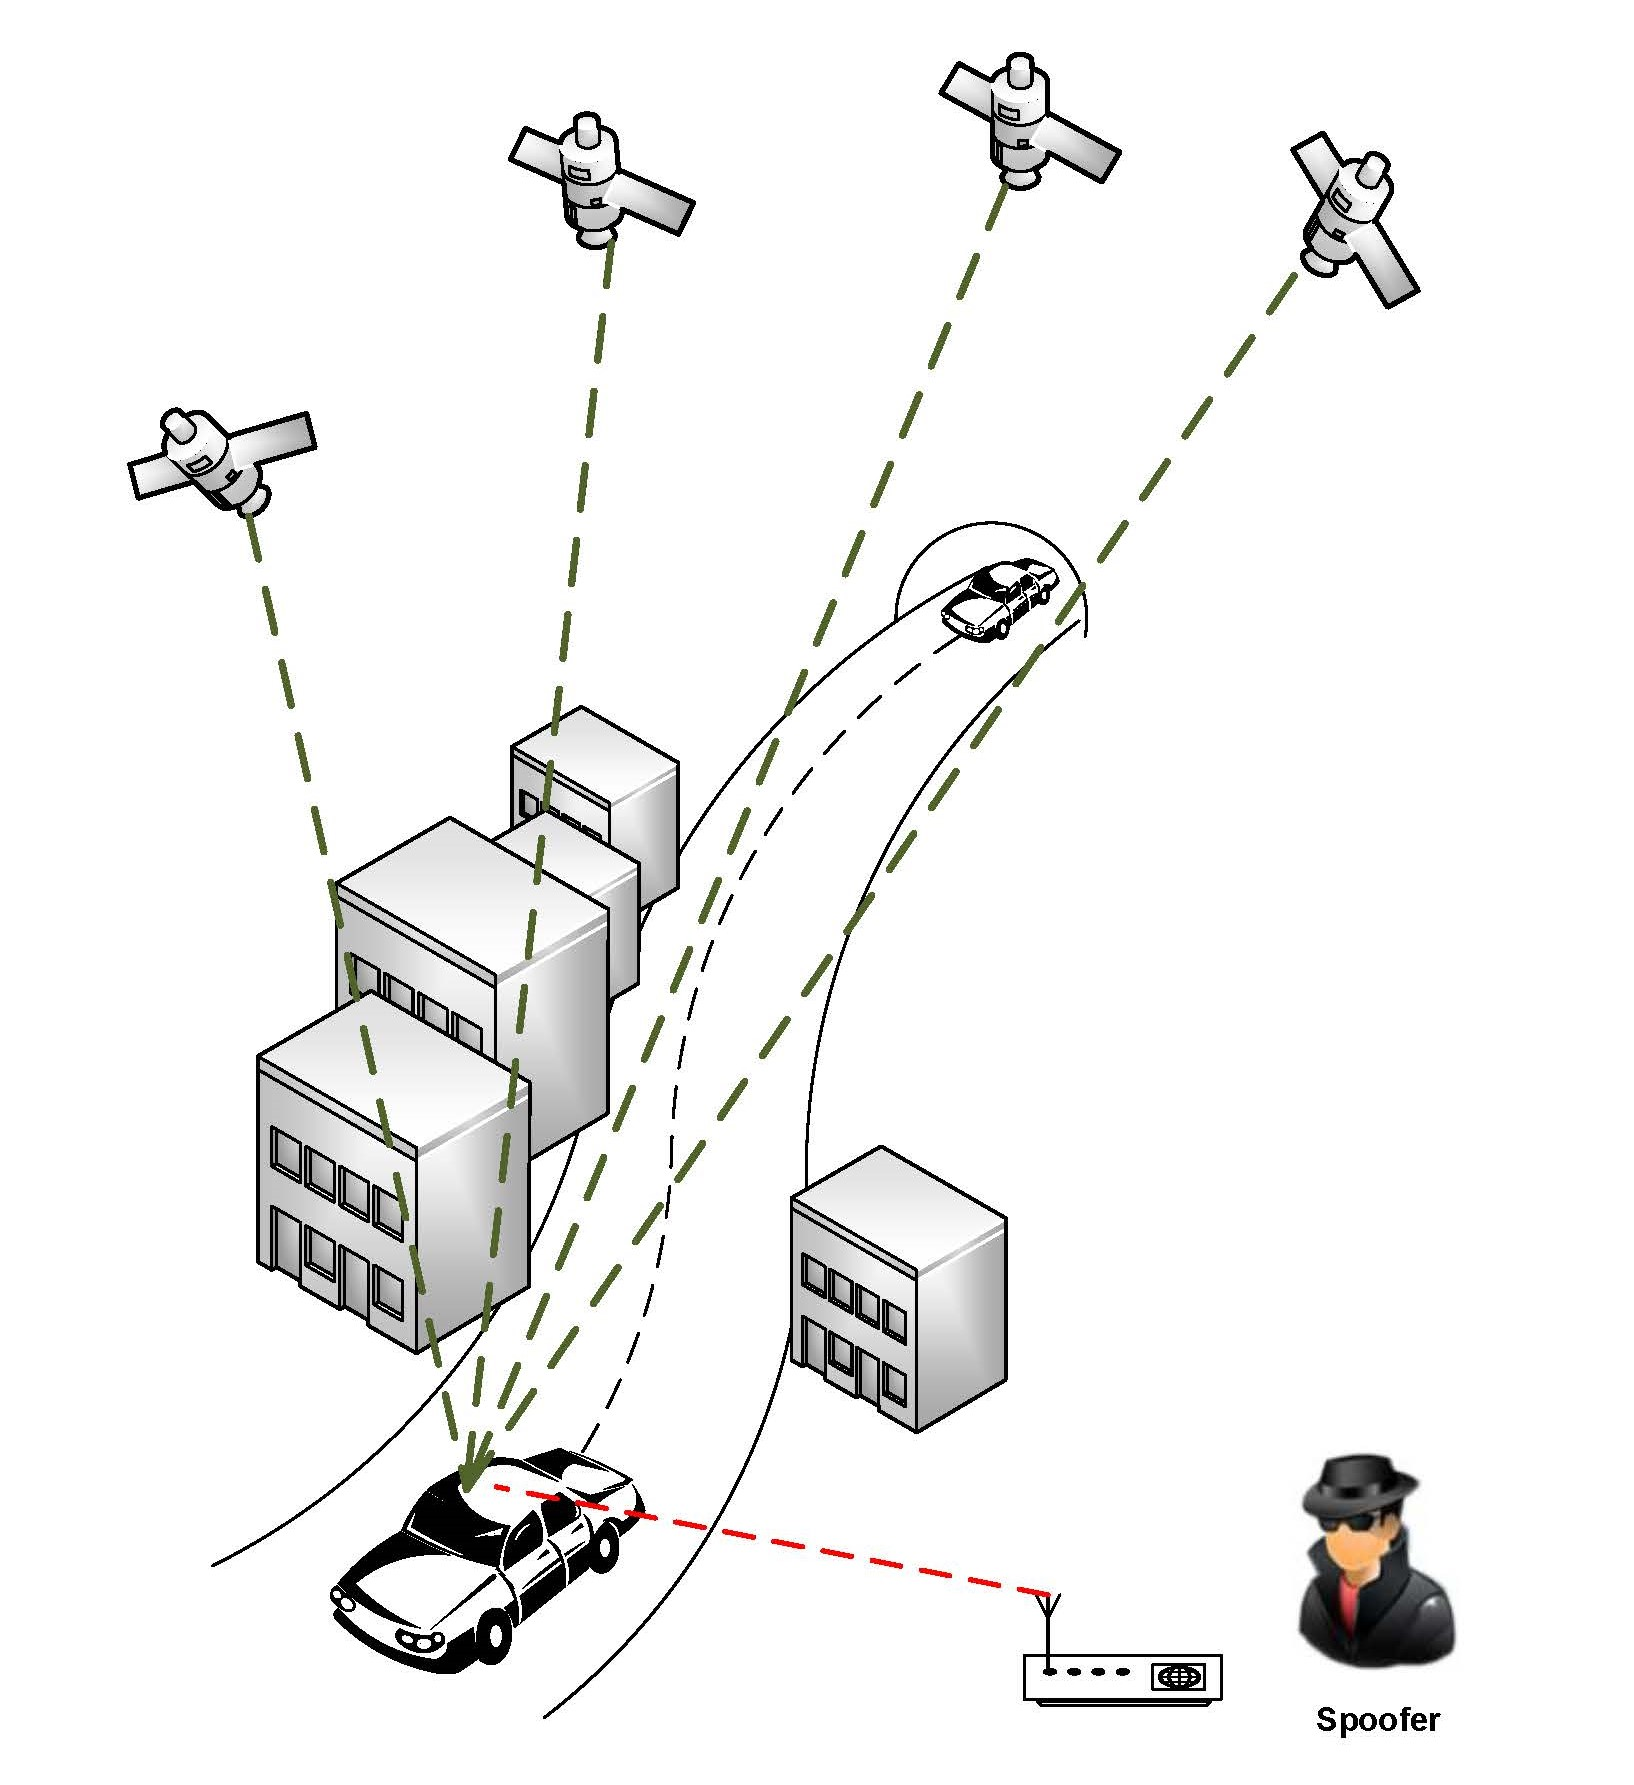
\includegraphics[scale=0.4]{images/Satnav_spoofing.jpg}
\caption{Un esempio di spoofing}
\label{fig: spoofing }
\end{figure}
Lo spoofing ad esempio, è stato dimostrato un mezzo in grado di forzare i droni o reindirizzare le navi, mentre alcuni luoghi ad alta sicurezza, come i confini internazionali interrotti, sono diventati noti per i segnali di spoofing che impediscono l'uso affidabile del navigatore satellitare nelle loro vicinanze. 

\subsection{Problemi dei sistemi GNSS}
Entriamo più nel dettaglio dei problemi di spoofing dei sistemi GNSS analizzando questa particolare tecnica. Considereremo da qui in avanti come sistema di posizionamento di riferimento il sistema di posizionamento Galileo\footnote{Il sistema di posizionamento Galileo è un sistema di posizionamento e navigazione satellitare civile, sviluppato in Europa come alternativa al GPS.}, visto che viene utilizzato da Intecs SpA per il loro sistema di certificazione della posizione. Informiamo il lettore che queste criticità si presentano anche negli altri sistemi di posizionamento come il GPS (Global Positioning System)\footnote{Il GPS (Global Positioning System) è un sistema di posizionamento e navigazione satellitare militare statunitense.}. Per individuare la posizione in cui ci troviamo si sfrutta un dispositivo di localizzazione che non fa altro che rimanere in ascolto dei segnali inviati dai satelliti e calcolare la distanza che intercorre tra sé e quest'ultimi, considerando il tempo di ricezione. Per effettuare un calcolo della posizione è necessario collegarsi ad almeno quattro satelliti, la cui posizione nello spazio è nota con precisione. Sfruttando i dati appena ottenuti è possibile calcolare l’intersezione delle quattro sfere immaginarie ed individuare la posizione del ricevitore. Spesso queste sfere si intersecheranno in parte invece che incontrarsi in un punto univoco e quindi il ricevitore calcolerà la posizione matematicamente più probabile. E' importante notare che il segnale dei satelliti catturato in una certa area è esattamente lo stesso di quello catturato nel raggio di alcune centinaia di km. Questo perché i satelliti si trovano distanti circa 23222 km dalla terra ed essendo posizionati molto in alto, coprono un'area molto estesa. Quello che cambia è il tempo con cui si riceverà il segnale dai satelliti trovandosi in due punti differenti. Un malintenzionato potrebbe catturare il segnale alla posizione A e ritrasmetterlo al dispositivo che si trova in posizione B accertandosi di essere in grado di oscurare il segnale dei satelliti in orbita. Un altro esempio a cui applicare questa tecnica di spoofing è con i pescherecci. Tipicamente hanno delle zone interdette dove non possono navigare e sono collegati ad un dispositivo GNSS per rilevare la posizione in tempo reale. Si può anche in questo caso sfruttare un escamotage: servirsi di un dispositivo che inganna il sistema che registra il segnale GNSS, facendogli registrare il segnale del sistema predisposto dall'attaccante invece del vero segnale acquisito dai satelliti.

\section{Che cos'è la Blockchain?}
La blockchain \cite{blockchain} (letteralmente "catena di blocchi") è una struttura dati condivisa e "immutabile". È definita come un registro digitale le cui transazioni sono raggruppate in "blocchi", concatenati in ordine cronologico, e la cui integrità è garantita dall'uso della crittografia. Il suo contenuto una volta scritto, non è più modificabile né eliminabile, a meno di non invalidare l'intera struttura. Le tecnologie basate su blockchain sono incluse nella più ampia famiglia dei Distributed Ledger, ossia sistemi che si basano su un registro distribuito, che può essere letto e modificato da più nodi di una rete. Non è richiesto che i nodi coinvolti conoscano l'identità reciproca o si fidino l'uno dell'altro perché, per garantire la coerenza tra le varie copie, l'aggiunta di un nuovo blocco è globalmente regolata da un protocollo di consenso eseguito da tutti i nodi. Una volta autorizzata l'aggiunta del nuovo blocco, ogni nodo aggiorna la propria copia privata. La natura stessa della struttura dati garantisce l'impossibilità di una sua manipolazione futura. Le caratteristiche che accomunano i sistemi sviluppati con le tecnologie blockchain e Distributed Ledger sono: digitalizzazione dei dati, decentralizzazione, tracciabilità dei trasferimenti, trasparenza/verificabilità, immutabilità del registro e programmabilità dei trasferimenti. Grazie a tali caratteristiche, la blockchain è considerata pertanto un'alternativa in termini di sicurezza, affidabilità, trasparenza e costi, alle banche dati e ai registri gestiti in maniera centralizzata da autorità riconosciute e regolamentate (pubbliche amministrazioni, banche, assicurazioni, intermediari di pagamento, ecc.).

% \subsection{Implementazione di una semplice Blockchain con Python}
% Diamo un'occhiata a una semplice implementazione di una blockchain in Python\footnote{Python è un linguaggio di programmazione dinamico orientato agli oggetti utilizzabile per molti tipi di sviluppo software.}. Innanzitutto, definiamo una funzione che chiamiamo bhash che, dato il timestamp e i dettagli (una stringa o un altro oggetto serializzabile) di una nuova transazione insieme all'hash della transazione precedente, calcola un nuovo hash utilizzando l'algoritmo SHA1:
% \begin{pythoncode}
% import hashlib, json, time

% def bhash (timestamp, details, prev_hash):
%     #la funzione dumps converte un oggetto Python in una stringa JSON
%     token = json.dumps([timestamp, details, prev_hash])
%     return hashlib.sha1(token).hexdigest())
% \end{pythoncode}
% Si noti che abbiamo usato il serializzatore json per combinare gli elementi insieme in una stringa che poi passiamo alla funzione hash SHA1 hash. La nostra scelta di serializzare in json è un dettaglio di implementazione e non l'unico modo per raggiungere l'obiettivo.
% Successivamente creiamo una classe Blockchain per incapsulare un elenco di blocchi:
% \begin{pythoncode}
% class Blockchain(object):
%     def __init__ (self, details='new-chain'):
%         self.blocks = [(time.time(), details, "")]
%     def record (self ,details, timestamp=None):
%         timestamp = timestamp or time.time()
%         #estraggo il campo hash dall'ultimo elemento della lista
%         prev_hash = self.blocks[-1][2]
%         new_hash = bhash(timestamp, details, prev_hash)
%         self.blocks.append((timestamp, details, new_hash))
% \end{pythoncode}
% La classe ha un costruttore, "init", che crea un elenco di blocchi e memorizza il primo blocco nell'elenco. Questo primo blocco contiene un timestamp iniziale e dettagli ma nessun hash. Nel caso di un bitcoin, questo memorizzerebbe informazioni sulla scoperta di una nuova unità e del suo proprietario.
% La classe ha anche un secondo metodo, "record", che, dati i dettagli di una nuova transazione e un timestamp opzionale (altrimenti calcolato automaticamente), li memorizza in un nuovo blocco. Questo viene fatto recuperando l'hash del blocco precedente da self.blocks [-1] [2] chiamando la funzione bhash e aggiungendo la tripla (timestamp, dettagli, new\_hash) all'elenco dei blocchi.
% Usiamo la nostra classe Blockchain creandone un'istanza, che chiamiamo "bc", e registriamo le transazioni rappresentate come stringhe autodescrittive:
% \begin{pythoncode}
% bc = Blockchain('A found 1 euro')
% bc.record('A gives 1 euro to B')
% bc.record('B gives 1 euro to C')
% bc.record('C gives 1 euro to D')
% \end{pythoncode}
% Quindi possiamo stampare i blocchi della blockchain con il comando seguente:
% \begin{pythoncode}
% print bc.blocks
% #output
% [(1495941516.704196, 'A found 1 euro', ""],
% (1495941516.704201, 'A gives 1 euro to B', 'a75a9227f...'),
% (1495941516.704277, 'B gives 1 euro to C', 'ca911be27...'),
% (1495941516.704290, 'C gives 1 euro to D', 'cb462885e...')]
% \end{pythoncode}
% L'ultimo hash è 'cb462885e...'. Affinché questa tecnologia funzioni, dobbiamo assicurarci di trasmettere l'ultimo hash e che ci siano alcune copie dell'intera blockchain memorizzate da parti diverse. Le parti in questo contesto sono i nodi di calcolo della rete peer-to-peer incaricati di registrare e archiviare le transazioni. Si tratta di un problema di rete che esula dall'ambito di questo articolo.
% È anche importante che ogni parte possa verificare l'integrità della blockchain. Questo può essere fatto facilmente utilizzando la funzione seguente:
% \begin{pythoncode}
% def verify (blockchain):
%     prev = blockchain.blocks[0]
%     for block in blockchain.blocks[1:]:
%         new_hash = bhash(block[0], block[1], prev[2])
%         if block[2] != new_hash: return False
%         prev = block
%     return True
% \end{pythoncode}
% Nel codice sopra, ripetiamo tutti i blocchi a partire dal secondo, ricalcoliamo ogni hash e poi lo confrontiamo con quello memorizzato in block[2]. Se il codice trova un hash che non corrisponde, restituisce False altrimenti restituisce True. Possiamo chiamare questo codice sulla nostra blockchain con:
% \begin{pythoncode}
% print verify(bc)
% #output
% True
% \end{pythoncode}
% Da un punto di vista tecnologico, c'è molto di più di questo nella rete Bitcoin. Esistono algoritmi per la distribuzione dei dati, per la sincronizzazione dei nodi, per l'archiviazione e l'interrogazione efficienti, per la risoluzione dei conflitti e così via, ma la tecnologia blockchain è al centro di esso\cite{8024092}.

\subsection{Blockchain nel progetto di tirocinio}
Per rendere più sicuro il sistema già esistente di certificazione della posizione, è stata utilizzata la tecnologia di Algorand \cite{algorand} attraverso l'introduzione di uno smart contract\footnote{Gli smart contract sono contratti che, una volta distribuiti, sono richiamabili in remoto da qualsiasi nodo nella blockchain di Algorand. Proprio come qualsiasi altro contratto, regola i termini e le condizioni di un accordo tra le parti.}, che ha reso possibile una maggiore sicurezza della comunicazione tra i componenti principali. Per quel che riguarda la sua creazione ed eliminazione, è stato deciso di concedere interamente ad Intecs SpA la possibilità di svolgere queste due operazioni. Sono anche state effettuate delle scelte implementative per impedire che lo smart contract non fosse in nessun modo modificato o eliminato da terzi. L'implementazione di questa procedura ha richiesto la creazione di un account Algorand ad uso esclusivo dell'azienda. Il lavoro di miglioramento del sistema di certificazione è stato svolto con l'obiettivo di conservare l'architettura del progetto di partenza.

\section{Breve riassunto dei capitoli successivi}
Nel capitolo \ref{2.statoarte} descriveremo i vari meccanismi di consenso delle diverse blockchain, della blockchain di Algorand e daremo un'introduzione al linguaggio PyTeal con cui vengono sviluppati gli smart contract. I meccanismi di consenso sono dei protocolli eseguiti all'interno di una rete distribuita e servono per validare le transazioni che sono state effettuate, ma possono servire anche per penalizzare chi decide di commettere irregolarità o chi non rispetta queste regole. La Proof of Work (PoW) e la Proof of Stake (PoS) sono i due algoritmi di consenso più famosi nel settore. Il primo utilizzato da Bitcoin, si basa sulla risoluzione di problemi matematici particolarmente complessi al fine di trovarne una soluzione chiamata "nonce"\footnote{Nonce è l’acronimo di “number only used once“, ovvero numero utilizzato una sola volta. Si riferisce al numero che un miner deve scoprire per poter risolvere un blocco nella blockchain.}. Il PoS, utilizzato da criptovalute come Solana e Cardano è un meccanismo di consenso in cui i validators garantiscono la validità delle operazioni effettuate impegnando una quota delle proprie criptovalute (dette "stake"). Algorand utilizza invece una versione diversa del PoS chiamata Pure Proof of Stake che sfrutta un protocollo di accordo bizantino per raggiungere il consenso tra gli utenti sulla prossima serie di transazioni. Vedremo anche i tool di sviluppo per Algorand, le operazioni richieste per collegarsi alla blockchain per ricercare informazioni e come scrivere direttamente su quest’ultima. Tramite Algod\footnote{Algod è uno strumento fornito da Algorand che approfondiremo nel capitolo \ref{2.statoarte}.} è possibile eseguire transazioni sulla blockchain mentre per supportare la ricerca si utilizza l'Indexer. Uno strumento rapido per creare e configurare un ambiente di sviluppo Algorand con Algod e Indexer prende il nome di Algorand Sandbox.

Daremo nel capitolo \ref{3.progetto iniziale} una descrizione del sistema di certificazione della posizione realizzato da Intecs SpA e introdurremo il sistema di posizionamento satellitare Galileo\cite{de2001galileo} per descrivere il suo funzionamento. Il progetto di partenza utilizza principalmente tre componenti: sistema centrale, sistema mobile e stazione di riferimento. Il sistema mobile e la stazione di riferimento acquisiscono nel solito istante, ogni 120 secondi, segnali cioè sequenze di bit dai satelliti Galileo in orbita sopra di loro. Per semplicità chiameremo l'insieme di questi segnali acquisiti da un solo dispositivo (sistema mobile o stazione di riferimento) "snapshot". Entrambe le componenti, ovvero il sistema mobile e la stazione di riferimento inviano lo snapshot catturato al sistema centrale che procederà con il confronto dei due snapshot per verificare la loro equivalenza.

Nel capitolo \ref{4.integriamo la blockchain} introdurremo il sistema degli smart contract, programmi che vengono archiviati sulla blockchain che possono generare transazioni di pagamenti, asset e possono anche memorizzare valori sulla blockchain. Sono in definitiva dei contratti che, una volta implementati, sono richiamabili in remoto. Per rendere più sicuro il sistema di certificazione della posizione già esistente è stato introdotto uno smart contract per far sì che alcune operazioni fossero più sicure e i dati di posizione immutabili.

Nel capitolo \ref{5.cli e intecs} daremo modo al lettore di capire come poter comunicare con il sistema di certificazione realizzato, introducendo due programmi fondamentali implementati con un'interfaccia a linea di comando: Cli e Intecs. Entrambi sono implementati con lo scopo di semplificare le varie operazioni (come il settaggio di parametri o la creazione ed eliminazione dello smart contract). Il programma Cli è univoco per ogni sistema mobile e nella prima versione (cli v1) rappresenta uno strumento per interfacciarsi al sistema mobile, poterlo interrogare e richiedere informazioni sugli snapshot ricevuti da quest'ultimo. Nella versione 2 (cli v2) il programma comunica direttamente con la blockchain di Algorand attraverso l'Indexer\footnote{Per ricercare informazioni nella blockchain di Algorand si fa uso di uno strumento chiamato Indexer V2. Lo scopo principale di questo indicizzatore è fornire un'interfaccia API REST di chiamate API per supportare la ricerca in Algorand Blockchain.} per estrarre informazioni dal campo nota di una particolare transazione che vedremo in seguito. 

Nel capitolo \ref{6.simulazione del progetto} mostriamo i vari step per poter avviare correttamente il progetto su un calcolatore\footnote{Il progetto è stato implementato e testato su sistema operativo Windows 10}. 

Infine, nel capitolo conclusivo (capitolo \ref{7.conclusioni}) mostriamo alcune implementazioni alternative rispetto al progetto realizzato e le features che non sono state realizzate per la mancanza di tempo a disposizione, che porterebbero però ad un maggior livello di sicurezza. Un'implementazione alternativa, analizzata solo concettualmente, che va nella direzione della filosofia di decentralizzazione che è intrinseca nella blockchain è quella di sfruttare una tecnologia decentralizzata anche per la memorizzazione dei dati. Nel progetto implementato, il sistema centrale archivia i file zip e JSON ricevuti dal sistema mobile e dalla stazione di riferimento internamente. Per evitare che questi file possano andare persi ed introdurre quindi una ridondanza, una soluzione sarebbe potuta essere quella di memorizzarli su IPFS\footnote{IPFS, acronimo di InterPlanetary File System, è file system decentralizzato, implementato con una rete peer-to-peer. Si tratta di un sistema per l'archiviazione e la condivisione di dati.}, un file system decentralizzato.

\chapter{Stato dell'arte}\label{2.statoarte}
\subsection{Storia della Blockchain}
La prima blockchain fu introdotta, nel 2008, ad opera di Satoshi Nakamoto (pseudonimo di un autore la cui identità è tuttora sconosciuta), e implementata l'anno seguente, con l'obiettivo di fungere da "libro mastro" (registro di tutte le transazioni) della nascente valuta digitale Bitcoin \cite{nakamoto2008bitcoin}. Nel 2009 la creazione di Satoshi Nakamoto, Bitcoin, fu utilizzata per la prima volta per l'acquisto di una pizza. Negli anni successivi, sono nate poi nuove blockchain che hanno preso spunto da questa \cite{blockchain}. Nel 2017, nasce anche Algorand, progetto basato sulla tecnologia blockchain per garantire transazioni scalabili, sicure e decentralizzate attraverso un meccanismo di consenso più rapido, efficiente e meno costoso rispetto a quelli già esistenti.

\subsection{Meccanismi di consenso}
I meccanismi di consenso sono dei procedimenti che avvengono all’interno di una rete distribuita e servono per mettere d’accordo i vari nodi sull’applicazione delle regole e definiscono il protocollo della rete. In questo caso vengono utilizzati per validare le transazioni che sono state effettuate, ma possono servire anche per poter penalizzare chi decide di commettere irregolarità o chi non rispetta queste regole \cite{8632190}.

\subsection{PoW vs PoS}
Il Proof of Work (PoW) e Proof of Stake (PoS) sono due tra gli algoritmi di consenso più famosi nel settore. Il primo è utilizzato da Bitcoin, mentre Proof of Stake è stato adottato da altre criptovalute come Algorand in una versione più efficiente.

\subsubsection{Proof of Work}
Il PoW (Proof of Work) si basa sulla risoluzione di problemi matematici particolarmente complessi da parte della rete, da cui il termine, letteralmente, “prova di lavoro”. Questo meccanismo di consenso sfrutta ciò che in gergo viene definito come “mining”: dei calcolatori molto potenti (detti anche miners) cercano di risolvere un problema matematico complesso al fine di poterne trovare una soluzione chiamata "nonce" e ricevere una ricompensa (ad esempio, un Bitcoin) per il lavoro svolto. Maggiore sarà la potenza di calcolo impiegata, maggiori saranno le possibilità di risolvere il problema matematico in quanto sarà maggiore il numero di tentativi al secondo effettuati. Il problema matematico proposto, infatti, può essere risolto solo per tentativi e il primo miner che trova la soluzione si aggiudica la ricompensa. Tuttavia, l’algoritmo di consenso PoW consente ai miners di convalidare un nuovo blocco e aggiungerlo alla blockchain solo se gli altri nodi della rete concordano con la soluzione fornita dal miner, ripetendo l’operazione risolta.

\subsubsection{Proof of Stake}
Il rapido sviluppo della tecnologia blockchain e delle loro numerose applicazioni emergenti ha ricevuto grande attenzione negli ultimi anni. Il meccanismo del consenso distribuito è la spina dorsale di una rete blockchain e svolge un ruolo chiave nel garantire la sicurezza, l'integrità e le prestazioni della rete. La maggior parte delle attuali reti blockchain ha implementato i meccanismi di consenso Proof of Work, in cui il consenso viene raggiunto attraverso processi di mining intensivi. Tuttavia, questo meccanismo presenta diverse limitazioni, ad esempio inefficienza energetica e scarsa scalabilità. Per superare questi problemi, è stato recentemente sviluppato un nuovo meccanismo di consenso, ovvero il Proof of Stake, che consente di ottenere il consenso dimostrando la proprietà della partecipazione. Questo meccanismo dovrebbe diventare una tecnologia all'avanguardia per le future reti blockchain \cite{nguyen2019proof}. Nel PoS il procedimento fisico attraverso il quale i supercomputer competono tra loro per risolvere problemi matematici complessi, cioè il mining, viene sostituito da un sistema in cui i cosiddetti "validators" garantiscono la validità delle operazioni effettuate impegnando una quota delle proprie criptovalute (dette “stake”). L’idea di base risiede nella necessità di evitare ingenti sprechi di energia e la competizione tra i nodi in merito alle capacità di calcolo. Il principale pregio dei sistemi di PoW risiede proprio nella necessità di impiegare innumerevoli risorse di elettricità ed energia per poter aumentare la potenza di calcolo e risolvere sempre più velocemente i problemi matematici proposti. Questo è ciò che rende il PoW un sistema ad alta affidabilità, in quanto i costi elevati associati al processo di mining rendono, se non impossibile, quantomeno improbabile che i miners investano le proprie risorse per ostacolare il network. Tuttavia, questa caratteristica costituisce anche il principale difetto del PoW \cite{pos}.

\section{Algorand: una Blockchain italiana}
Algorand è una blockchain pubblica completamente permissionless e decentralizzata fondata dal matematico, crittografo e informatico italiano Silvio Micali. Le blockchain permissionless sono quelle in cui chiunque può partecipare al processo di validazione delle transazioni e diventare un nodo della rete. Gli utenti non necessitano l'approvazione di alcuna autorità per unirsi alla rete e chiunque può utilizzare la blockchain per effettuare transazioni e partecipare alla generazione dei blocchi. I dati sono pubblici, quindi tutti i partecipanti possono leggere ogni singolo blocco e hanno facoltà di scrivere una transazione in un blocco futuro. Bitcoin è stata la prima blockchain permissionless che ha ispirato molti a ridefinire l'algoritmo di consenso in un ambiente decentralizzato. In ogni caso, la natura del protocollo Proof of Work ha fatto sì che la capacità di generare i blocchi si sia negli anni progressivamente concentrata tra un numero ristretto di miners. Questo ha portato alla separazione degli utenti in due distinte classi: gli utenti ordinari che utilizzano Bitcoin e i miner professionisti che traggono profitto dalla generazione di nuovi blocchi, questo a causa del fatto che per molti utenti il costo per partecipare alla generazione dei blocchi è divenuto troppo alto \cite{algorand2}.

\subsection{Pure Proof of Stake}
Algorand garantisce che gli utenti non abbiano mai visioni divergenti delle transazioni confermate, anche in presenza di attacchi e se la rete è temporaneamente partizionata. Al contrario, le criptovalute esistenti consentono fork temporanei e quindi richiedono molto tempo, nell'ordine di un'ora, per confermare le transazioni con elevata confidenza. Algorand utilizza un nuovo protocollo di accordo bizantino (BA)\footnote{Il problema dei generali bizantini, in inglese Byzantine Agreement (acronimo di BA) è un problema informatico che consiste nel trovare un accordo, comunicando solo tramite messaggi, tra componenti diversi nel caso in cui siano presenti informazioni discordanti.} per raggiungere il consenso tra gli utenti sulla prossima serie di transazioni. Per scalare il consenso a molti utenti, Algorand utilizza un nuovo meccanismo basato su funzioni casuali verificabili. In questo modo gli utenti sono in grado di verificare privatamente se sono stati selezionati per partecipare alla BA per concordare la prossima serie di transazioni e per includere una prova della loro selezione nei loro messaggi di rete. Nel protocollo BA di Algorand, gli utenti non mantengono alcuno stato privato, il che consente ad Algorand di sostituire i partecipanti immediatamente dopo aver inviato un messaggio. Ciò attenua gli attacchi mirati ai partecipanti scelti dopo che la loro identità è stata rivelata. Valutando le prestazioni di Algorand su 1.000 macchine virtuali EC2\footnote{Amazon Elastic Computer Cloud abbreviato in Amazon EC2, è una parte centrale della piattaforma di cloud computing Amazon Web Services (AWS) di Amazon, che permette agli utenti di affittare macchine virtuali sulle quali eseguire le proprie applicazioni} e simulando fino a 500.000 utenti, i risultati sperimentali mostrano che questa blockchain è in grado di confermare le transazioni in meno di un minuto, raggiungere 125 volte il throughput\footnote{Il throughput è il numero vero di transazioni al secondo che la blockchain è in grado di gestire.} di Bitcoin e non subire quasi nessuna penalità per il ridimensionamento a più utenti.

\subsubsection{Consenso da parte del comitato}
BA ottiene la scalabilità scegliendo un comitato, un piccolo gruppo di rappresentanti selezionati casualmente dall'insieme totale di utenti, per eseguire ogni fase del proprio protocollo. Tutti gli altri utenti osservano i messaggi di protocollo, che consentono loro di apprendere il blocco concordato. BA sceglie i membri del comitato in modo casuale tra tutti gli utenti in base al peso di quest'ultimi. Ciò consente ad Algorand di garantire che una parte sufficiente dei membri del comitato sia onesta. Tuttavia, fare affidamento su un comitato crea la possibilità di attacchi mirati contro i membri del comitato prescelto. Per evitare che un avversario prenda di mira i membri del comitato, BA seleziona i membri in modo privato e non interattivo. Ciò significa che ogni utente nel sistema può determinare in modo indipendente se è stato scelto per far parte del comitato, calcolando una funzione (VRF \cite{814584}) sfruttando la propria chiave privata e delle informazioni pubbliche dalla blockchain. Se la funzione indica che l'utente è stato scelto, restituisce una breve stringa che dimostra l'appartenenza al comitato di questo utente ad altri utenti, che l'utente può includere nei suoi messaggi di rete. Poiché la selezione dell'appartenenza non è interattiva, un avversario non sa quale utente scegliere come target finché quell'utente non inizia a partecipare a BA. Infine, un avversario può prendere come bersaglio un membro del comitato una volta che quel membro ha inviato un messaggio in BA. BA mitiga questo attacco richiedendo ai membri del comitato di parlare solo una volta. Pertanto, una volta che un membro del comitato invia il suo messaggio (esponendo la sua identità a un avversario), il membro del comitato diventa irrilevante per BA. BA raggiunge questa proprietà evitando qualsiasi stato privato (eccetto la chiave privata dell'utente), che rende tutti gli utenti ugualmente in grado di partecipare, ed eleggendo un nuovo comitato per ogni fase del protocollo di accordo bizantino \cite{algorand-bizantine}.

\section{Gli smart contract}
In questa sezione, vedremo cosa sono e come si possono implementare gli smart contract. In generale, sono programmi che vengono archiviati sulla blockchain ed eseguiti quando vengono soddisfatte determinate condizioni; possono generare transazioni di pagamenti e asset, possono anche memorizzare valori sulla blockchain. Quando lo smart contract viene creato, la rete restituirà un application-id (ID) univoco, il quale può quindi essere utilizzato per effettuare chiamate (Application Call) a quest'ultimo. Lo smart contract avrà anche un indirizzo Algorand univoco che viene generato da questo ID che gli permette di fungere da garante tra due o più soggetti per lo scambio di beni quando una certa condizione è stata soddisfatta. In Algorand, gli smart contract possono essere scritti in TEAL o PyTeal; il primo (TEAL) è un linguaggio Turing-completo\footnote{Un linguaggio di programmazione è Turing-complete se la sua semantica permette di implementare una qualsiasi macchina di Turing.} simile ad assembler, il secondo (PyTeal) è una libreria Python per la generazione di programmi TEAL che fornisce una sintassi comoda e familiare.

\subsection{Variabili locali e globali}
Nella fase di creazione di uno smart contract è necessario specificare le variabili utilizzate, che possono essere di due tipologie: stringhe di byte o interi senza segno. Le variabili devono essere specificate sia a livello globale che locale e sono dichiarate come nell'esempio di seguito:

\begin{pythoncode}
#dichiarazione dello stato di memoria dell'applicazione (immutabile)
local_ints = 1
local_bytes = 1
global_ints = 0
global_bytes = 1
global_schema = transaction.StateSchema(global_ints, global_bytes)
local_schema = transaction.StateSchema(local_ints, local_bytes)
\end{pythoncode}

Il numero di variabili che possono essere memorizzate è limitato in base a come è stato creato il contratto la prima volta. Nell'esempio sopra viene creato uno smart contract con due variabili: una locale di tipo intero senza segno e una globale di tipo stringa. Lo spazio della chiave\footnote{La chiave è intesa come il nome della variabile.} è limitato a 64 byte mentre la chiave più il valore può arrivare al massimo a 128 byte totali. L’archiviazione globale è formata dai dati che vengono specificatamente memorizzati sulla blockchain a livello globale. I valori di archiviazione locale vengono archiviati nell'account che ha aderito allo smart contract con la fase di opt-in\footnote{La fase di opt-in avvia la partecipazione di un utente allo smart contract.}.

\subsection{Tipi di smart contract}
Gli smart contract si dividono in due grandi categorie: smart contract detti anche stateful contract e smart signature chiamati anche stateless contract.

\subsubsection{Smart Contract (stateful contract)}
 Gli smart contract sono contratti che, una volta implementati, sono richiamabili in remoto. Una volta distribuita, l'istanza on-chain del contratto prende il nome di "applicazione" a cui viene assegnato un ID univoco. Gli smart contract possono accedere ai valori della blockchain, come i saldi dei conti e i parametri di configurazione delle risorse. Sono in grado anche di eseguire transazioni come parte dell'esecuzione della logica. Ogni applicazione ha un account associato che può contenere Algo (criptovaluta di Algorand)\footnote{L'Algo è la moneta  della rete principale di Algorand, la MainNet.} o ASA (Algorand Standard Asset \cite{asa}). Nel tipo di contratto stateful una certa quantità di spazio di archiviazione sulla blockchain viene utilizzata per memorizzare valori (globalmente o localmente). L'archiviazione dei valori locali si riferisce alla memorizzazione dei valori nel saldo del conto dell'account se l'account ha aderito allo smart contract. Lo storage globale invece è un dato che viene specificamente archiviato sulla blockchain per lo smart contract, a livello globale. In Algorand, uno smart contract è composto da due programmi:
 \begin{itemize}
 \item Approval-Program: è responsabile di tutte le chiamate ad eccezione del Clear-Program.
 \item Clear-Program: questo tipo di programma viene utilizzato per rimuovere lo smart contract dall'account Algorand che lo chiama.
 \end{itemize}
 Entrambi i programmi possono avere successo o fallire, a seconda della logica con cui sono stati implementati. Se una variabile globale o locale viene modificata e il programma ha esito negativo, le modifiche di stato non verranno applicate.
 
\subsubsection{Smart Signature (stateless contract)}
Gli smart signature sono piccoli programmi che vengono inviati come parte di una transazione e valutati al momento dell'invio che contengono la logica utilizzata per firmare le transazioni. Sebbene la logica nello smart signature sia archiviata nella blockchain come parte della risoluzione della transazione, la logica non è richiamabile da remoto. Quando la logica viene inviata a un nodo, l'AVM (Algorand virtual machine)\footnote{L'Algorand virtual machine (AVM) gira su ogni nodo della blockchain di Algorand e si tratta di una macchina virtuale che valuta gli smart contract e gli smart signature rispetto alle transazioni con cui vengono chiamati.} valuta se la condizione codificata dalla logica della smart signature è verificata o meno; nel caso non sia verificata, la transazione associata non verrà eseguita. Una transazione firmata con uno smart signature viene valutata da un nodo Algorand utilizzando la macchina virtuale Algorand (AVM). L'obiettivo principale di questi contratti è quello di approvare (Approve) o rifiutare (Reject) le transazioni.

\subsubsection{Metodi dell'Applicazione}
Le chiamate agli smart contract avvengono utilizzando le transazioni. Di seguito, vediamo tutti i tipi di chiamate:
\begin{enumerate}
    \item Create: metodo che distribuirà l'app. La creazione dell'applicazione restituisce un application-id.
    \item Opt-In: uno user-account (utente Algorand) utilizza questa transazione per iniziare a partecipare ad uno smart contract. La partecipazione attiva l'utilizzo della memoria locale (local storage) dell'utente. Ovviamente per partecipare è necessario conoscere l'application-id che viene restituito dopo la creazione dello smart contract.
    \item Call(NoOp): l'utente può ora iniziare ad usare l'applicazione dopo che nel punto 2 ha partecipato allo smart contract. Questo metodo serve per chiamare/eseguire l'Approval-Program\footnote{L'Approval-Program è responsabile dell'elaborazione di tutte le chiamate allo smart contract, ad eccezione della clear-call eseguita con il Clear-Program. Questo programma è responsabile dell'implementazione della maggior parte della logica dello smart contract.}.
    \item Read State: chiunque può leggere lo stato globale di un'applicazione o lo stato locale di un'applicazione di un certo account utilizzando le API\footnote{API è l'abbreviazione di interfaccia di programmazione delle applicazioni (application programming interface), ovvero un insieme di definizioni e protocolli per la creazione e l'integrazione di software applicativi.}.
    \item UpdateApplication: transazione da eseguire per aggiornare i programmi TEAL di uno smart contract (ovvero l'Approval-Program e il Clear-Program). Il creatore può aggiornare l'Approval-Program usando il metodo di update (ovviamente se l'attuale Approval-Program lo consente). Attenzione, in realtà chiunque può aggiornare il programma, per questo motivo se non si desidera che questo accada è necessario aggiungere del codice per gestire questa situazione, come nel seguente esempio:
    
    \begin{pythoncode}
    program = Assert(Global.creator_address()==Txn.sender())
    print(compileTeal(program, Mode.Application)
    \end{pythoncode}
    % \lstinputlisting[label= updateapp1, caption= Esempio, language=python, basicstyle=\small]{listing/sourceCode/updateapp1.py}
    In alternativa possiamo costruire un codice che restituisca sempre 0 quando viene effettuata una chiamata all'applicazione per impedire a chiunque di aggiornare il codice, come in quest'altro esempio:

    \begin{pythoncode}
    is_not_update = Seq( Return(Int(1))
    program = If (
     OnComplete.UpdateApplication == Txn.on_completion(),
     Return(Int(0)),
     is_not_update
    )
    print(compileTeal(program, Mode.Application)
    \end{pythoncode}
    % \lstinputlisting[label= updateapp2, caption= Esempio, language=python, basicstyle=\small]{listing/sourceCode/updateapp2.py}
    
    \item Close out: l'utente può interrompere l'uso dell'applicazione inviando una transazione di chiusura. Ciò rimuoverà lo stato locale per questa applicazione dell'account dell'utente. Gli utenti utilizzano quindi questa transazione per chiudere la loro partecipazione allo smart contract. Questa chiamata può non riuscire in base alla logica TEAL, impedendo all'account di rimuovere lo smart contract dal balance record (record di saldo).
    \item Delete: transazione che elimina l'applicazione. Chiunque può eliminare uno smart contract, se non si vuole ciò bisogna modificare la logica del programma.
    \item Clear State: simile a Close Out ma la transazione eliminerà sempre lo smart contract dal record del saldo del conto (account balance record) indipendentemente che il programma abbia esito positivo o negativo.
\end{enumerate}

\subsection{Buona programmazione degli smart contract}
Quando si lavora con TEAL per sviluppare smart contract, è necessario seguire alcune linee guida. Ad esempio è consigliato verificare sempre che la proprietà RekeyTo di qualsiasi transazione sia impostata su ZeroAddress a meno che lo smart contract non sia specificamente coinvolto in un'operazione di rekeying. Il rekeying consente di modificare la propria chiave privata senza la necessità di modificare il proprio indirizzo pubblico. Nella maggior parte delle blockchain invece, quando è necessario modificare una chiave privata perchè compromessa, è necessario aprire un nuovo account e spostare le risorse dal vecchio account al nuovo. Per informazioni sulle linee guida è sufficiente visitare la pagina ufficiale \cite{guidelines}.

\section{PyTeal}
Com'è stato accennato in precedenza, PyTeal è una libreria Python per la generazione di programmi TEAL che fornisce una sintassi comoda e familiare.

\subsection{Tipi}
Un'espressione PyTeal può far riferimento a uno dei seguenti tipi di dato: 
\begin{itemize}
    \item uint64, interi senza segno a 64 bit
    \item byte slice, stringhe di bytes
\end{itemize}
Sia i valori delle variabili locali che globali per il contratto corrente possono essere modificati dal codice dello smart contract. 
Vediamo alcuni semplici esempi di codice in grado di creare, aggiornare e eliminare valori nello stato locale o globale. 

\begin{pythoncode}
from pyteal import *

#  variabili globali
program = App.globalPut(Bytes("MyKey"), Int(50))
program = App.globalGet(Bytes("MyKey"))
program = App.globalDel(Bytes("MyKey"))

#  variabili locali
program = App.localPut(Int(0), Bytes("MyKey"), Int(50))
program = App.localGet(Int(0), Bytes("MyKey"))
program = App.localDel(Int(0), Bytes("MyKey"))
print (compileTeal(program, Mode.Application))
\end{pythoncode}
% \lstinputlisting[label= variabili, caption= le variabili, language=python, basicstyle=\small]{listing/sourceCode/localglobalVariable.py}

\subsection{Oggetti di tipo Txn}
Di seguito, descriviamo gli oggetti che è possibile utilizzare nel nostro contratto intelligente:

\begin{enumerate}
    \item Txn: è un oggetto (in particolare un'istanza) che contiene la transazione corrente da valutare per vedere se rispetta lo smart contract
    \item GTxn: è invece un oggetto che contiene un gruppo di transazioni in fase di valutazione (è un'istanza di TxnGroup).
    \item InnerTxn: è un'istanza di TxnObject, contiene la transazione interna inviata più di recente.
\end{enumerate}

\subsection{Seq}
Espressioni multiple possono essere presenti in una sequenza.

\begin{pythoncode}
program = Seq (
    App.globalPut(Bytes("count"), App.globalGet(Bytes("count"))+Int(1)),
    Approve()
)
\end{pythoncode}
% \lstinputlisting[label= seq, caption= Esempio dell'uso di Seq, language=python, basicstyle=\small]{listing/sourceCode/seq.py}

Questo programma conta semplicemente le volte in cui è stato eseguito cioè imposta il conteggio della chiave "count" sul valore che detiene attualmente a cui sommo uno e infine approva. Sfrutta il fatto che App.globalGet restituirà 0 se provi a cercare una chiave che non esiste ancora.

\subsection{Condizioni base: if, then, else, elseif}
\begin{pythoncode}
program = Seq (
    if (App.globalGet(Bytes("count"))==Int(100))
    .then (
        #100esimo chiamante di questa app
        App.globalPut(Bytes("100thCaller"), Txn.sender())
    )
    .else (
        App.globalPut(Bytes("not100thCaller"), Txn.sender())
    ),
    App.globalPut(Bytes("count"), App.globalGet(Bytes("count"))+Int(1)),
    Approve(),
)
\end{pythoncode}

Il programma appena mostrato utilizza tre variabili globali: "count" di tipo uint64, "100thCaller" e "not100thCaller", entrambe di tipo byte slice. Una volta chiamato, il programma controlla che il valore associato a "count" sia uguale a 100 e se questa condizione è verificata, scrive su "100thCaller" l'indirizzo pubblico del mittente della transazione, altrimenti quest'ultimo indirizzo viene scritto sulla variabile "not100Caller". Infine, viene incrementato di uno il valore di "count".

\subsection{Subroutines}
In PyTeal le subroutine sono essenzialmente funzioni o pezzi di codice che possono essere inserite in una funzione Python. E' necessario aggiungere  il decoratore di subroutine e dichiarare il tipo restituito. Di seguito, vediamo un esempio:

\begin{pythoncode}
@Subroutine(TealType.uint64)
def isEven(i) :
    return i%Int(2) == Int(0)
App.globalPut(Bytes("value_is_even"), isEven(Int(10)))
\end{pythoncode}
% \lstinputlisting[label= subroutine1, caption= Esempio subroutine, language=python, basicstyle=\small]{listing/sourceCode/subroutine1.py}

\begin{pythoncode}
@Subroutine(TealType.uint64)
def recursiveisEven(i) :
    return (
        if (i == Int(0)
        .Then ( Int(1)
        .ElseIf ( i == Int(1))
        .Then ( Int(0))
        .Else (recursiveisEven( i-Int(2))
\end{pythoncode}
% \lstinputlisting[label= subroutine2, caption= Esempio subroutine risorsiva, language=python, basicstyle=\small]{listing/sourceCode/subroutine2.py}

Quello che accade è che il codice in fase di compilazione viene archiviato. Ogni volta che viene invocato il metodo, si va alla riga della subroutine, si esegue la funzione e infine si ritorna alla riga del codice in cui eravamo precedentemente.

\subsection{Inner Transaction}
A partire da AVM 1.0 le applicazioni possono creare ed eseguire singole transazioni chiamate "inner-transaction". Le transazioni interne consentono alle applicazioni stateful (smart contract) di avere molti degli effetti di una transazione di primo livello ma la principale differenza è che queste non sono firmate.

\section{Sviluppare con Algorand}
In questa sezione, analizzeremo i tool di sviluppo per Algorand, come collegarsi alla blockchain per ricercare informazioni e come poter scrivere su quest'ultima attraverso le transazioni. Prima di iniziare con gli argomenti appena elencati introduciamo quali sono le tipologie di rete pubbliche disponibili e le loro differenze. In Algorand esistono quattro reti pubbliche: MainNet, BetaNet, TestNet e DevNet. La prima (MainNet) è la rete principale di Algorand con asset a valore reale, inclusa la valuta nativa di Algorand: l'Algo. TestNet rispecchia MainNet in termini di versione del suo protocollo (ovvero software) e la valuta si chiama Algos, disponibile tramite un dispenser, presenta il blocco genesi diverso, il che significa che lo stato dei conti e la distribuzione dei fondi sono differenti. BetaNet è la blockchain in cui verranno rilasciate nuove funzionalità a livello di protocollo per i test iniziali. Pertanto, la qualità e le funzionalità potrebbero non essere definitive e gli aggiornamenti del protocollo e i riavvii della rete sono comuni. DevNet è una rete basata su nightly build\footnote{Le nightly build o build notturne vengono solitamente rilasciate quotidianamente e solitamente di notte, a significare il termine di una giornata lavorativa.}. \cite{algorand_network}.

\subsection{Algorand Sandbox}
La Sandbox di Algorand è un modo rapido per creare e configurare un ambiente di sviluppo Algorand con Algod\footnote{Tramite Algod è possibile eseguire transazioni alla blockchain per la creazione di uno smart contract, effettuare chiamate a quest’ultimo, fare aggiornamenti e cancellazioni e molto altro ancora.} e Indexer\footnote{L'Indexer è lo strumento fornito da Algorand per ricercare informazioni nella blockchain.} ed è disponibile sul portale GitHub\footnote{GitHub è un servizio di hosting per progetti software.}. E' uno strumento fornito da Algorand che semplifica per lo sviluppatore il processo di configurazione di un nodo Algorand in un ambiente containerizzato. Con containerizzazione intendiamo il raggruppamento di codice software e di tutti i relativi componenti necessari, come librerie, framework e altre dipendenze, in modo che risultino isolate in un proprio contenitore che chiamiamo "container". Questo metodo consente di eseguire in modo uniforme il software o l'applicazione contenuta nel container in qualsiasi ambiente e infrastruttura, indipendentemente dal sistema operativo eseguito. Il container costituisce una sorta di bolla, un ambiente di elaborazione circostante all'applicazione, che la mantiene indipendente da ciò che la circonda \cite{containerization}. Per iniziare ad utilizzare la Sandbox è necessario prima clonare la repo da terminale, con il comando:
\begin{pythoncode}
git clone https://github.com/algorand/sandbox.git
\end{pythoncode}
Accertarsi poi che Docker-Compose sia installato e che Docker Desktop sia in esecuzione.

\subsubsection{Configurazioni integrate}
Le seguenti configurazioni vengono fornite di default con Sandbox e possono essere utilizzate eseguendo il comando \textit{./sandbox up <config>} dal terminale, assicurandosi di trovarsi all'interno della cartella "sandbox" appena scaricata. \\ \\
L'elenco delle configurazioni (<config>) di rete privata disponibili sono:
\begin{itemize}
    \item release - build di sviluppo stabile di algod e ramo principale di Indexer.
    \item nightly - build di sviluppo stabile di algod e il ramo di sviluppo di Indexer.
    \item beta - build beta di algod e ramo di sviluppo di Indexer.
    \item dev - ramo di sviluppo di algod e Indexer, la costruzione di algod richiede un po' di tempo, quindi questo avvio sarà più lento rispetto alle altre configurazioni di rete privata.
\end{itemize}
Esiste anche una configurazione (<config>) per ciascuna delle reti di lunga durata:
\begin{itemize}
    \item mainnet
    \item testnet
    \item betanet
    \item devnet
\end{itemize}

\subsubsection{Come usare la Sandbox}
Per avviare la Sandbox e inizializzare la rete privata predefinita, viene utilizzato il comando \textit{./sandbox up}.

\subsection{Algod}
Un'applicazione si connette alla blockchain di Algorand tramite un client Algod che richiede un indirizzo IP e un token Algod valido da un nodo Algorand connesso alla rete con cui prevede di interagire. Tramite Algod è possibile eseguire transazioni alla blockchain per la creazione di smart contract, effettuare chiamate a quest'ultimo, fare aggiornamenti e cancellazioni. E' poi possibile creare asset, aggiornarli, eliminarli o effettuare transazioni ad altri account Algorand. In poche parole è lo strumento che utilizziamo per poter interagire con la blockchain. L'operazione di lettura della blockchain invece la si fa tramite l'indicizzatore (Indexer).

\subsubsection{Instanziare Client Algod SDK}
Per utilizzare il client Algod e potersi connettere alla rete della Testnet è necessario aver avviato la Sandbox con il comando \textit{./sandbox up testnet}.
Fatto ciò, vediamo il codice Python per collegarsi effettivamente al client:
\begin{pythoncode}
from algosdk.v2client import algod

algod_address = "http://localhost:4001"
algod_token = 
"aaaaaaaaaaaaaaaaaaaaaaaaaaaaaaaaaaaaaaaaaaaaaaaaaaaaaaaaaaaaaaaa"
algod_client = algod.AlgodClient(algod_token, algod_address)
\end{pythoncode}

\subsubsection{Alternativa alla Sandbox}
Un'alternativa all'Algorand Sandbox per comunicare con la rete MainNet, BetaNet e TestNet è Purestake: un servizio che offre un’interfaccia sicura per permettere l'utilizzo di Algod e dell’Indexer. Nella versione standard gratuita si ha accesso a tutti i tipi di reti (TestNet, BetaNet e MainNet) e possono essere eseguite 500.000 richieste al giorno, 30 query Algod e 10 query Indexer al secondo. Per poter usufruire del servizio è obbligatorio registrarsi in quanto si richiede una chiave privata (nell'esempio chiamata "my-private-key") per far funzionare il client, fornita dopo l'iscrizione. Di seguito si mette a disposizione il codice base per il collegamento ad Algod della TestNet utilizzando il linguaggio di programmazione Python:
\begin{pythoncode}
headers = {
"X-API-Key": "my-private-key",
}
algod_client = algod.AlgodClient("",
"https://testnet-algorand.api.purestake.io/ps2", headers)
\end{pythoncode}

\subsubsection{Direttiva per Docker}
Per utilizzare Algod (istanziato con la Sandbox) all'interno di un container Docker dobbiamo sostituire "localhost" in algod\_address con "host.docker.internal", poiché vogliamo che il container acceda alla porta host \textit{sandbox 4001}. Mostriamo di seguito questo concetto per maggiore chiarezza:

\begin{pythoncode}
from algosdk.v2client import algod

algod_address = "http://host.docker.internal:4001"
algod_token = 
"aaaaaaaaaaaaaaaaaaaaaaaaaaaaaaaaaaaaaaaaaaaaaaaaaaaaaaaaaaaaaaaa"
algod_client = algod.AlgodClient(algod_token, algod_address)
\end{pythoncode}

\subsection{Indexer}
Per ricercare informazioni nella blockchain di Algorand si fa uso di uno strumento chiamato Indexer V2 (versione 2). Lo scopo principale di questo indicizzatore è fornire un'interfaccia API REST di chiamate API per supportare la ricerca in Algorand Blockchain. Le API REST dell'indicizzatore recuperano i dati blockchain da un database PostgreSQL che deve essere popolato utilizzando la stessa istanza dell'indicizzatore o un'istanza separata dell'indicizzatore che deve connettersi al processo Algod di un nodo Algorand in esecuzione per leggere i dati del blocco [vedi figura \ref{fig: indexer}]. Questo nodo deve essere anche un nodo di archiviazione per rendere possibile la ricerca nell'intera blockchain. L'indicizzatore fornisce una serie di chiamate API REST per la ricerca di transazioni, conti, asset e blocchi sulla blockchain. Ognuna di queste chiamate fornisce anche diversi parametri di filtro per supportare il perfezionamento delle ricerche \cite{algorand_indexer}.

\begin{figure}[!h]
\centering
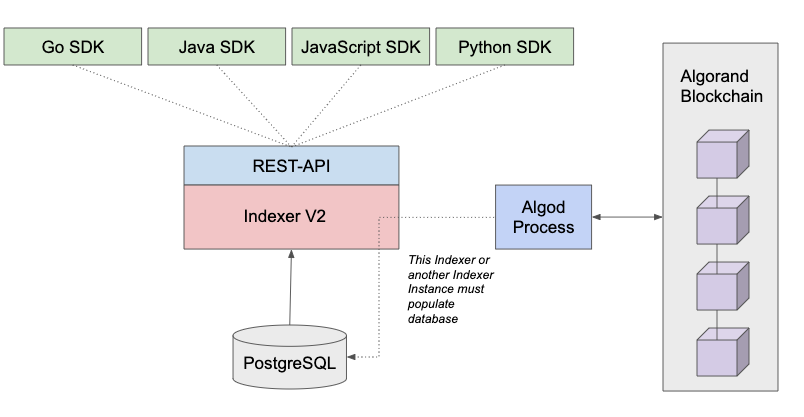
\includegraphics[scale=0.4]{images/indexerv2.png}
\caption{Architettura Indexer V2}
\label{fig: indexer}
\end{figure}

\subsubsection{Instanziare Client Indexer SDK}
La Sandbox non ha lo scopo di fornire un Indexer di TestNet, visto che il suo scopo è di creare un nodo rapido per lo sviluppo di:
\begin{itemize}
    \item una nuova rete privata con un Indexer (che è molto conveniente per la maggior parte dei casi)
    \item un rapido nodo non di archiviazione per TestNet senza Indexer
\end{itemize}

Se si desidera un Indexer TestNet, è necessario eseguire sia un nodo TestNet di archiviazione che un nodo Indexer. Quest'operazione è piuttosto lunga visto che ci vorrà circa una settimana per recuperare tutte le informazioni dalla blockchain e rendere tutto operativo. Per semplificare questo processo è stato utilizzato PureStake: un servizio che offre un'interfaccia sicura all'Indexer V2 di Algorand. Di seguito, si mostra il codice per potersi collegare a questo servizio correttamente:

\begin{pythoncode}
from algosdk.v2client import indexer
headers = {
"X-API-Key": "my-private-key",
}
# instantiate indexer client
myindexer = indexer.IndexerClient("", "https://testnet-algorand.api
.purestake.io/idx2", headers)
\end{pythoncode}

\section{Docker}
Docker è un popolare software libero progettato per eseguire processi informatici in ambienti isolabili, minimali e facilmente distribuibili chiamati container, con l'obiettivo di semplificare i processi di deployment di applicazioni software \cite{docker}. Lo scopo di Docker è quindi quello di rendere più facile la creazione, il deploy e l'esecuzione di applicazioni utilizzando i container. I container consentono allo sviluppatore di pacchettizzare una applicazione con tutte le parti necessarie (le librerie e altre risorse correlate) e consegnarla appunto come un unico pacchetto \cite{docker1}.

\subsection{Le immagini}
Un'immagine Docker è un modello in sola lettura che definisce il container. L'immagine contiene il codice che verrà eseguito, incluse le definizioni per le librerie e le dipendenze necessarie. Un container Docker è un'immagine Docker in esecuzione. Per creare un immagine è necessario creare un particolare file chiamato “Dockerfile”. Il Dockerfile può essere considerato come un manuale di assemblaggio per le immagini. Il suo scopo però non si esaurisce qui. Oltre a specificare come deve essere costruita un’immagine, descrive anche la modalità (di default) con la quale verrà avviato un container a partire da essa. Le istruzioni dichiarate nel Dockerfile verranno eseguite in ordine e, in buona approssimazione, per ognuna di esse verrà generato un layer.

\subsection{Persistenza dei dati}
I container sono pensati per essere distrutti e ricreati più volte a partire dalla stessa immagine. Questo approccio fa parte del concetto di “infrastruttura immutabile” che garantisce lo stesso container ad ogni nuovo deploy. Viene da se che quando si presenta l’esigenza di persistere delle informazioni oltre il ciclo di vita del container o tra più container è necessario avere qualche soluzione che stia al di fuori del container stesso. A dire il vero, è possibile persistere le informazioni anche su un container fino al momento in cui questo container viene distrutto. Tuttavia non è la migliore strategia se poi queste informazioni devono essere disponibili anche al di fuori del contesto di quel singolo container. Per gestire la persistenza dei dati, Docker fornisce due soluzioni:
\begin{itemize}
    \item Volumes: i volumi sono uno spazio creato al di fuori dello Union File System del container che può essere acceduto da più container. Possono essere connessi a più container che ci interagiranno mediante un percorso locale definito da noi.
    \item Bind Mounts: alla stregua dei mount classici di linux, un bind mount è una condivisione di una cartella.
    Con questa tipologia di persistenza, andiamo a condividere una cartella dell’host con il container specificando anche in questo caso a quale path deve accedere in locale per poterci avere accesso \cite{docker_persistenza}.
    \end{itemize}

\subsection{Dockerfile}
Un Dockerfile è un semplice file di testo che, con una sintassi semplice e coincisa, ci permette di esprimere le personalizzazioni che vogliamo apportare ai vari template affinché questi possano diventare delle immagini su misura per noi. 
Di seguito presentiamo le istruzioni più importanti che andranno a comporre questo file.
\begin{description} 
\item[FROM] Tra le tante istruzioni disponibili, FROM è sicuramente quella più importante, nonchè l'unica che non può mai mancare all'interno di ogni Dockerfile. Essa permette di specificare un'immagine di base da cui partire per derivare la nostra immagine personalizzata.
\item[ENV]  Questa istruzione offre la possibilità di impostare variabili di ambiente valide per tutto il contesto di esecuzione di un Dockerfile.
 \item[RUN] Il comando RUN ha lo scopo di eseguire una o più istruzioni definite in formato bash in un nuovo layer. Di fatto aggiungendo un blocco immutabile all’immagine. Se è stato indicato di voler utilizzare Debian come immagine base, possiamo utilizzare l'istruzione RUN per installare un pacchetto tramite il classico comando apt-get.
 \item [CMD] Passiamo ora all’ultima istruzione necessaria per costruire una build, ovvero CMD. CMD è l’istruzione di default per l’esecuzione di un container. Fondamentalmente significa che al run di un container a partire dall’immagine che stiamo definendo, verrà invocata questa istruzione. Ogni Dockerfile ben formato dovrebbe avere al massimo una sola occorrenza di CMD. Ad ogni modo, in presenza di invocazioni multiple, verrà utilizzata solo l’ultima di esse. RUN agisce in fase di build apportando modifiche all’immagine, mentre il comando CMD specifica cosa fare quando viene avviato un container a partire da un’immagine che a tutti gli effetti è già sigillata.
 \item [COPY/ADD] Ci sono poi i comandi COPY e ADD che si occupano di copiare qualcosa dal filesystem dell’host all’interno dell’immagine. Questi due comandi hanno molto in comune. La differenza principale tra i due sta nel fatto che ADD è una sorta di COPY più evoluto, che permette di copiare risorse anche passando un url o decomprimendo direttamente un file qualora venisse riconosciuto come file compresso. 
 \item [EXPOSE] I container, di default non hanno nessuna porta aperta verso l’esterno ed è proprio qui che interviene EXPOSE. Per poter esporre una porta all’esterno, è necessaria la pubblicazione di quella porta relativamente al container che viene istanziato a partire dall’immagine che stiamo descrivendo. Le modalità previste sono due: aperture selettive o aperture generiche. Vediamo solo la prima modalità visto che risulta la più comune. Nell'apertura selettiva, si specifica quindi, quale porta ed eventualmente su quale protocollo viene pubblicata una porta del container verso l’esterno.
 \begin{pythoncode}
 EXPOSE 80/tcp
 EXPOSE 80/udp
 \end{pythoncode}
 Qualora non fosse specificato la porta verrà esposta di default sul protocollo TCP \cite{dockerfile}.
 \item [Altre istruzioni] Sopra sono state mostrate le istruzioni più comuni che sono anche quelle utilizzate all'interno del progetto \cite{dockerbuilder}.
\end{description} 

\subsection{Docker Compose}
Quando si utilizza Docker in modo estensivo, la gestione di diversi contenitori diventa rapidamente difficile da gestire. Docker Compose è uno strumento che ci aiuta a superare questo problema e a gestire facilmente più contenitori contemporaneamente. Con Compose, si utilizza un file YAML per configurare i servizi dell'applicazione. Quindi, con un solo comando, si creano e avviano tutti i servizi. In breve, Docker Compose funziona applicando molte regole dichiarate all'interno di un singolo file di configurazione docker-compose.yml. Quasi ogni regola sostituisce un comando Docker specifico in modo che alla fine dobbiamo solo eseguire:
\begin{pythoncode}
docker-compose up
\end{pythoncode}
Nel file docker-compose.yml è necessario specificare la versione del formato file Compose, almeno un servizio e, facoltativamente, volumi e reti:
\begin{pythoncode}
version: "3.7"
services:
  ...
volumes:
  ...
networks:
  ...
\end{pythoncode}

\subsubsection{Servizi}
I servizi si riferiscono innanzitutto alla configurazione dei container. Ad esempio, consideriamo un'applicazione Web dockerizzata composta da un front-end, un back-end e un database: probabilmente divideremmo quei componenti in tre immagini e li definiremmo come tre diversi servizi nella configurazione:
\begin{pythoncode}
services:
  frontend:
    image: my-vue-app
    ...
  backend:
    image: my-springboot-app
    ...
  db:
    image: postgres
    ...
\end{pythoncode}

\subsubsection{Avvio}
Possiamo avviare il file docker-compose.yml e cioè creare e avviare i container, le reti e i volumi definiti nella configurazione, con il comando seguente:
\begin{pythoncode}
docker-compose up
\end{pythoncode}

\subsubsection{Arresto}
Per interrompere in sicurezza i servizi attivi, possiamo utilizzare il comando \textit{stop}, che conserverà container, volumi e reti, insieme ad ogni modifica apportata agli stessi:
\begin{pythoncode}
docker-compose stop
\end{pythoncode}
Per poterlo riavviare, possiamo semplicemente utilizzare il comando:
\begin{pythoncode}
docker-compose start
\end{pythoncode}
Per resettare lo stato del nostro progetto (distruggerà tutto con la sola eccezione dei volumi esterni), si utilizza il comando:
\begin{pythoncode}
docker-compose down
\end{pythoncode}
\cite{docker-compose}

\subsection{Uso di Docker}
Creando container e avviandoli tramite il docker-compose.yml è possibile farli comunicare senza dover aprire le varie porte. Nel caso si abbia invece la necessità di dover comunicare con un container dall'esterno (ad esempio tramite browser) bisognerà necessariamente aprire manualmente le porte del container.

\chapter{Il progetto iniziale}\label{3.progetto iniziale}
Intecs SpA com'è stato accennato nel capitolo introduttivo, ha sviluppato un sistema di certificazione della posizione basato su tecnologia GNSS/SDR. In questo capitolo daremo una panoramica del sistema di certificazione approfondendo le scelte implementative.

\section{Il sistema Galileo}
Prima di addentrarci nel progetto vero e proprio diamo maggiori dettagli sul sistema di posizionamento Galileo, utilizzato da Intecs SpA come sistema di posizionamento satellitare.

\subsection{Che cos'è Galileo?}
Il sistema di posizionamento Galileo è un sistema di posizionamento e navigazione satellitare civile, sviluppato in Europa come alternativa al Global Positioning System (NAVSTAR GPS), controllato invece dal Dipartimento della Difesa degli Stati Uniti d'America. Il sistema fornisce un grado di accuratezza di alcuni centimetri nelle tre direzioni, l'entrata in servizio inizialmente fu prevista a fine 2019 ma è stata poi anticipata al 15 dicembre 2016. Il sistema conta 30 satelliti artificiali orbitanti di cui 24 operativi più 6 di scorta.

\subsection{Storia}
I primi sistemi di posizionamento satellitare, furono sviluppati in piena guerra fredda per applicazioni militari e il loro utilizzo civile è ancora oggi, in linea di principio, subordinato alle necessità di impiego militare. La necessità di rompere il monopolio USA di un servizio su scala globale ha spinto l'Europa a varare il progetto Galileo.

\subsection{Principi di funzionamento}
Un sistema di posizionamento globale satellitare come Galileo è un sistema basato su una costellazione di satelliti artificiali in grado di fornire con estrema precisione le coordinate geografiche (longitudine, latitudine, quota)\footnote{La longitudine è la coordinata geografica che specifica quanto la posizione di un punto sulla superficie terrestre si trovi ad est oppure ad ovest rispetto al Meridiano di Greenwich assunto come riferimento. La latitudine è la coordinata geografica che specifica quanto la posizione di un punto sulla superficie terrestre si trovi a nord o a sud dell’equatore. L’altitudine o quota è la distanza verticale di un oggetto dal livello del mare, ossia l’altezza sul livello del mare.} e la velocità di qualsiasi mezzo fisso o mobile in ogni punto in prossimità della superficie Terra e nell'atmosfera, con continuità temporale. Ciascun satellite trasmette continuamente dei segnali codificati contenenti varie informazioni come i dati orbitali, che servono ad un ricevitore satellitare per il calcolo della posizione del satellite stesso e un riferimento temporale per la determinazione degli istanti esatti di trasmissione dei segnali stessi.

\subsection{Calcolo della posizione}
Il principio di funzionamento del sistema Galileo (e anche del GPS) è sostanzialmente semplice: si tratta di determinare la distanza da 4 satelliti (S1, S2, S3, S4) la cui posizione nello spazio è nota con precisione e, mediante opportuni passaggi matematici, determinare la propria posizione. Quando 4 satelliti sono misurati contemporaneamente, l’intersezione delle 4 sfere immaginarie individua la posizione del ricevitore [vedi figura \ref{fig: gps_triangolazione }]. Queste sfere si intersecheranno in parte invece che incontrarsi in un punto univoco e quindi il ricevitore calcolerà una approssimazione della posizione calcolata in modo probabilistico.
\begin{figure}[h]
\centering
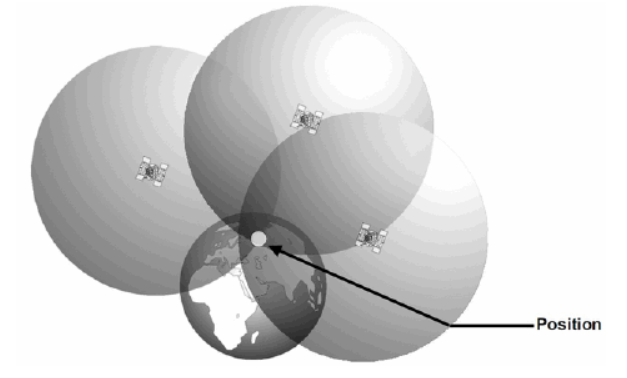
\includegraphics[scale=0.6]{images/gps_triangolazione.png}
\caption{Un esempio di triangolazione dei satelliti}
\label{fig: gps_triangolazione }
\end{figure}
La distanza del ricevitore dai satelliti viene determinata misurando lo scarto temporale che intercorre tra la trasmissione di una sequenza di bit inviata a Terra da ciascun satellite (trasmissione unidirezionale, tempi misurati da orologi atomici controllati e sincronizzati tra loro). Per utilizzare tale sistema in maniera unidirezionale, è necessario sapere con precisione l'istante di tempo in cui il codice viene trasmesso e misurare l'istante d'arrivo del segnale al ricevitore mediante l'uso di orologi esattamente sincronizzati. 

\subsection{Di cosa si occupa il sistema di certificazione realizzato da Intecs?}
Il sistema di certificazione della posizione verifica che lo snapshot registrato dal sistema mobile e dalla stazione di riferimento nello stesso momento sia equivalente. Se acquisiscono lo stesso snapshot, possiamo ipotizzare che nessuno stia cercando di attuare tecniche di spoofing e siamo in grado di considerare attendibile la posizione del dispositivo mobile, certificandolo. Sia il sistema mobile che la stazione di riferimento acquisiscono segnali da un certo numero di satelliti. Il confronto dei segnali viene eseguito su ogni satellite in comune cioè confrontando il segnale del solito satellite acquisito sia dal sistema mobile che dalla stazione di riferimento. Se alla fine del processo di confronto, un solo satellite in comune risulta non autenticato (cioè i due segnali sono diversi), la posizione non sarà certificata. In particolare, per poterla certificare è necessario che almeno quattro satelliti in comune siano autenticati. I segnali catturati dalla stazione di riferimento potrebbero essere "spoofati". Per risolvere questo problema si possono utilizzare più stazioni di riferimento per poter fare un check distribuito e su queste condizioni si considera totalmente sicura questa componente.

\section{Architettura del progetto iniziale}
L'architettura del sistema di certificazione della posizione realizzato da Intecs SpA è formata da tre componenti: sistema mobile, sistema centrale e stazione di riferimento. 
\begin{figure}[h]
\centering
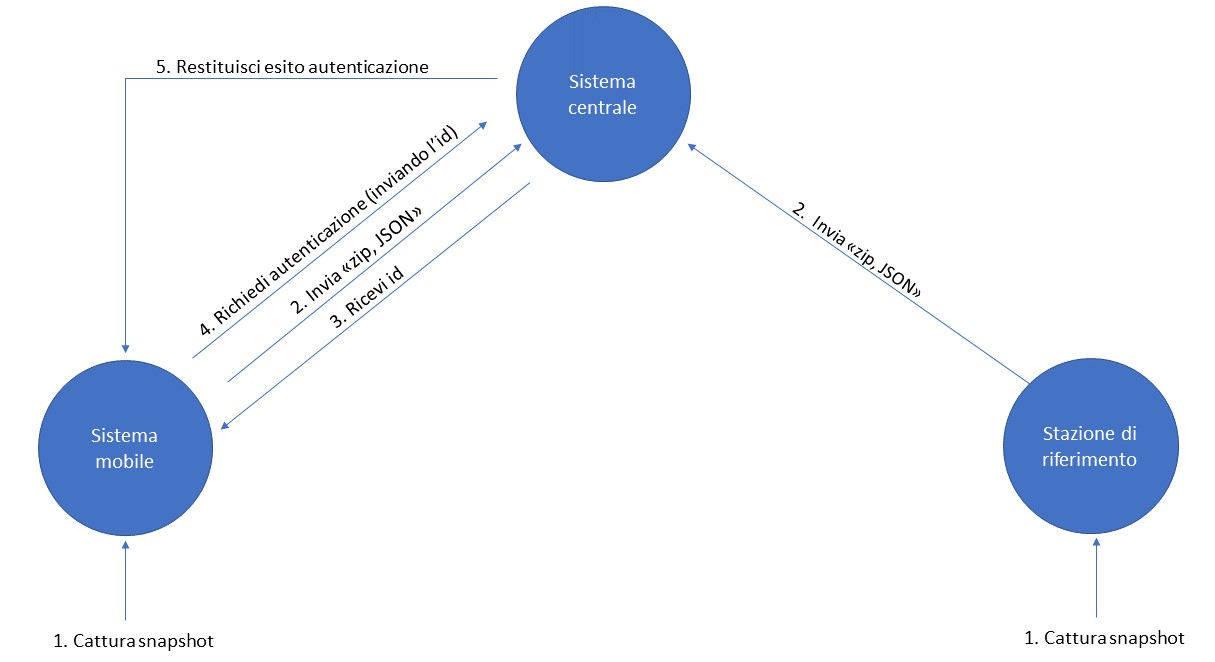
\includegraphics[scale=0.5]{images/schema progetto base.jpg}
\caption{Architettura del sistema di certificazione della posizione}
\label{fig: architetturabase }
\end{figure}
Sia il sistema mobile che la stazione di riferimento acquisiscono ogni 120 secondi\footnote{L'acquisizione dello snapshot può essere settato manualmente, ma non può essere mai inferiore ai 60 secondi.} un segnale\footnote{Questo tipo di segnale è rappresentato con una sequenza di bit.} da ognuno dei satelliti Galileo a cui si collegano, sfruttando un ricevitore satellitare. Lo snapshot catturato\footnote{Per semplicità chiameremo l'insieme di questi segnali acquisiti da un solo dispositivo (sistema mobile o stazione di riferimento) "snapshot".} viene salvato in un file all'interno di un archivio zip e utilizzato per calcolare i dati di posizione (altitudine, latitudine, longitudine ed altri parametri che per semplicità non considereremo) che assieme al timestamp sono inseriti in un file JSON. Il timestamp (o time-reference)\footnote{Un timestamp è una sequenza di caratteri che rappresentano una data e/o un orario per accertare l’effettivo avvenimento di un certo evento.} ha una precisione del millisecondo e rappresenta la data e l'ora dell'istante in cui il sistema mobile e la stazione di riferimento iniziano ad acquisire il segnale dai satelliti. Le due componenti sono sincronizzate con un orologio atomico in modo che la ricezione dello snapshot avvenga nel solito istante. L'acquisizione dello snapshot ha una durata di 5 secondi. Dopo la ricezione da parte del sistema mobile e dalla stazione di riferimento dello snapshot, entrambi inviano al sistema centrale due file rispettivamente: il file zip e il file JSON, attraverso una richiesta di tipo http-multipart\footnote{Una richiesta http-multipart è una richiesta http che i client http costruiscono per inviare file e dati su un server http.}. Il sistema mobile dopo l'invio dei due file, riceverà un messaggio di conferma ricezione contenente l'id univoco associato al file zip appena inviato, che utilizzerà per richiedere la certificazione dello snapshot al sistema centrale. A questo punto, il sistema centrale è in grado di verificare che i due snapshot siano uguali, comparandoli, il che significa confrontare ogni segnale (file binario) riferito al solito satellite in comune, sfruttando un algoritmo di allineamento delle due sequenze di bit. Questo allineamento è necessario visto che anche se gli snapshot vengono catturati dalle due macchine nello stesso istante e per lo stesso periodo di tempo (un intervallo di 5 secondi) gli orologi potrebbero non essere correttamente sincronizzati come in figura \ref{fig: algoritmoallineamento }]. In questo particolare esempio infatti, il sistema mobile inizia a catturare il segnale dal satellite Galileo "GSAT0103 - David" un istante prima rispetto a quello catturato dalla stazione di riferimento.
 \begin{figure}[h]
\centering
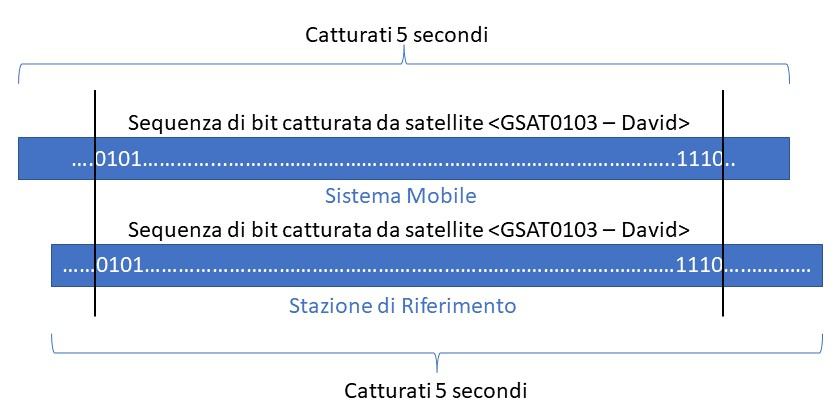
\includegraphics[scale=0.5]{images/grafico allineamento snapshot.jpg}
\caption{Un esempio di funzionamento dell'algoritmo di allineamento tra due snapshot}
\label{fig: algoritmoallineamento }
\end{figure}

\subsection{Database del Sistema Centrale}
Il sistema centrale ha due database interni: un Object Storage (gestito con MinIO\footnote{MinIO è un object storage le cui API sono compatibili con Amazon S3, un servizio offerto da Amazon Web Services (AWS) che fornisce storage di oggetti tramite un'interfaccia di servizio Web.}) che contiene gli snapshot e un database dei Metadati (gestito con Elasticsearch\footnote{Elasticsearch è un motore di ricerca e analisi dei dati distribuito basato su Apache Lucene.}) contenente i file JSON. Quando il sistema centrale riceve la richiesta http-multipart dal sistema mobile e dalla stazione di riferimento riceve sia il file zip che il JSON e inserisce il file zip (che contiene un file binario detto snapshot) nell'Object Storage. La procedura di inserimento restituisce un identificatore che rappresenta l'id univoco del file zip appena inserito nel database, questo file viene successivamente aggiunto ad un record assieme al file JSON e immagazzinato nel database dei metadati. La figura \ref{fig: salvataggioinfo } sottostante schematizza la spiegazione appena data.
\begin{figure}[!h]
\centering
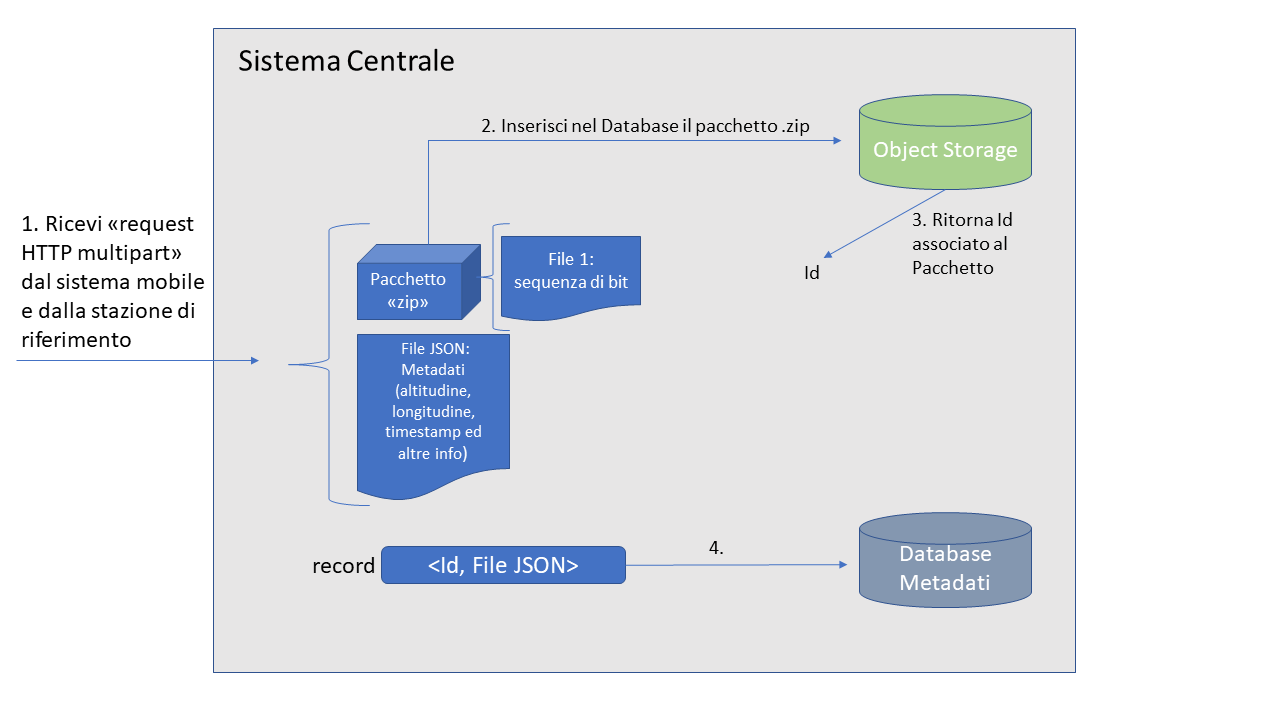
\includegraphics[scale=0.4]{images/Foto4.png}
\caption{Un esempio di salvataggio del file zip e del JSON}
\label{fig: salvataggioinfo }
\end{figure}

\subsection{Come confrontare gli snapshot}
Il confronto degli snapshot è un'operazione che avviene non appena il sistema centrale riceve dal sistema mobile la richiesta di autenticazione attraverso l'invio dell'id associato allo snapshot. Sfruttando l'id, il sistema centrale estrae il pacchetto zip nell'object storage e il record <id,json> dal proprio database dei metadati. Successivamente dal pacchetto zip viene estratto il file snapshot.bin. Si estrae il timestamp dal file JSON e si ricerca nel database dei metadati il record riferito alla stazione di riferimento. A questo punto viene confrontato, tramite l'algoritmo di allineamento degli snapshot visto sopra, lo snapshot del sistema mobile con quello della stazione di riferimento [vedi figura \ref{fig: ricercasnapshot }].
\begin{figure}[!h]
\centering
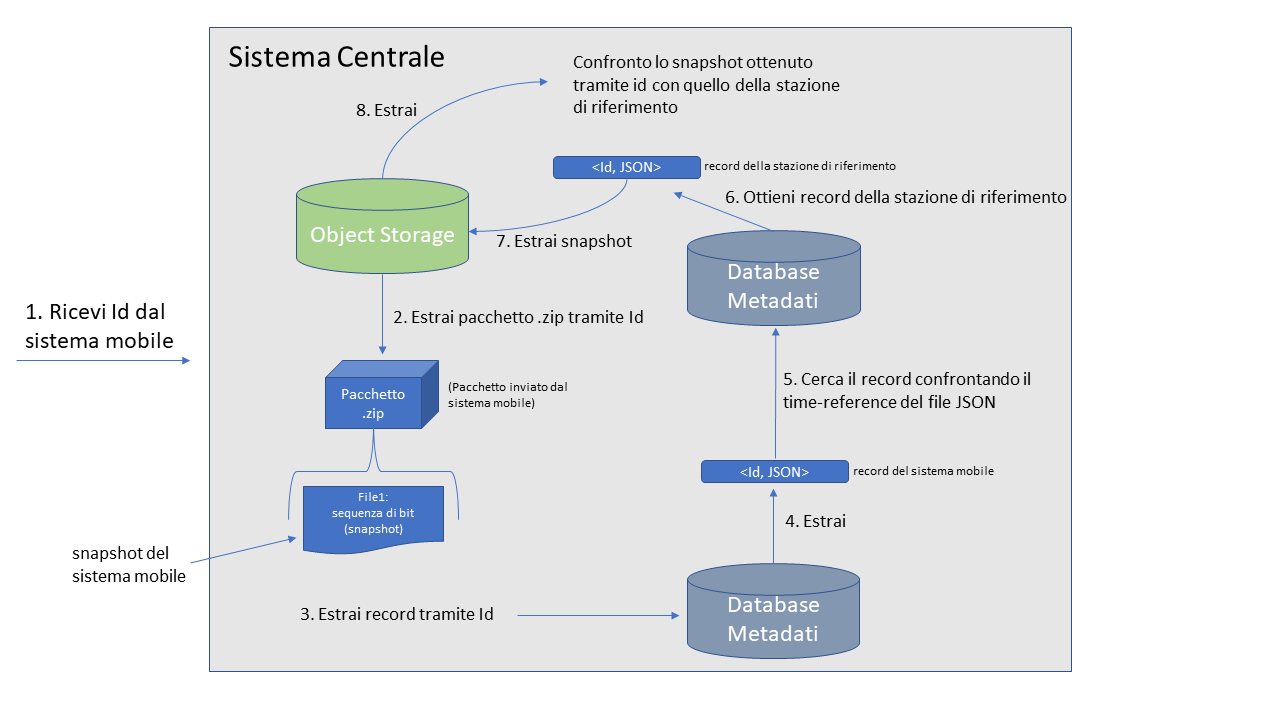
\includegraphics[scale=0.5]{images/Foto5.png}
\caption{Ricerca snapshot da id}
\label{fig: ricercasnapshot }
\end{figure}

\chapter{Integrazione con la Blockchain}\label{4.integriamo la blockchain}
Al fine di rendere più sicuro il sistema già esistente di certificazione della posizione, è stata introdotta la tecnologia blockchain di Algorand, che consente di rendere più sicure alcune operazioni immagazzinando i dati di posizione in blockchain rendendoli così immutabili.

\section{Introduzione}
Il nuovo progetto ha mantenuto parte dell'architettura di base con l'aggiunta di uno smart contract per aumentare i livelli di sicurezza. La sua gestione è controllata da Intecs SpA e sono state elaborate scelte implementative per impedire che lo smart contract non sia in nessun modo modificato o eliminato da terzi\footnote{Lo smart contract è memorizzato in blockchain e non sarà mai realmente eliminato dalla struttura dati. La procedura di eliminazione imposta la variabile booleana "Deleted" associata ai dettagli dello smart contract a True e questo rende impossibile richiamare i metodi dello smart contract.}. La necessità è stata quindi quella di creare un account Algorand ad uso esclusivo dell'azienda, la quale si occuperà anche della gestione di un altro account dello stesso tipo per il sistema centrale. Quest'ultimo componente (il sistema centrale) è unico ed ha il compito di chiamare due metodi dello smart contract: compare\_hash e validate\_snapshot. Infine, sarà necessario anche creare un account Algorand per ogni sistema mobile per poter richiamare il metodo insert\_local\_hash. 

\subsection{Il problema della certificazione degli snapshot}
Durante lo studio della tecnologia Algorand sono state evidenziate alcune incongruenze su quello che doveva essere uno degli obiettivi principali. Si è accennato nell'introduzione che lo scopo del tirocinio fosse quello di certificare la posizione direttamente su blockchain. Questa soluzione non risulta possibile, visto che, per certificare due snapshot è necessario applicare l'algoritmo di allineamento visto nel capitolo precedente e l'implementazione di quest'ultimo nello smart contract risulterebbe troppo complicato e costoso a livello computazionale. Per questa ragione il confronto viene eseguito direttamente dal sistema centrale.

\subsection{Antenna: una componente per simulare la ricezione degli snapshot}
L'antenna è una componente che simula il dispositivo di localizzazione del segnale satellitare (chiamato anche ricevitore) connesso al sistema mobile e alla stazione di riferimento. Nel sistema di base, il sistema mobile e la stazione di riferimento catturano lo snapshot attraverso i satelliti Galileo e calcolano la propria posizione sfruttando queste informazioni (maggiori spiegazioni sono date nel capitolo \ref{3.progetto iniziale}). Il sistema mobile e la stazione di riferimento sono dotati di un orologio atomico perfettamente sincronizzato che permette l'acquisizione dei segnali satellitari nel solito istante. A cadenza di 120 secondi acquisiscono i segnali dai satelliti e nell'istante in cui iniziano a farlo, registrano un timestamp\footnote{Un timestamp è una sequenza di caratteri che rappresentano una data e/o un orario per accertare l’effettivo avvenimento di un certo evento.} che sarà lo stesso per entrambe le macchine. Il timestamp ci risulta utile visto che, a partire dal timestamp associato allo snapshot del sistema mobile è possibile individuare lo snapshot catturato dalla stazione di riferimento e confrontare le due sequenze. Nel nuovo sistema sviluppato che introduce la blockchain, non è possibile che i sistemi mobili e le stazione di riferimento abbiano un orologio atomico sincronizzato visto che si tratta di un prototipo che simula il funzionamento del sistema di certificazione della posizione che non si collega realmente ai satelliti Galileo. Per trovare una soluzione a questo problema, è stata implementata la componente antenna che a cadenza regolare di 120 secondi acquisisce un timestamp e uno snapshot (sequenza di lettere e numeri generato casualmente) e lo invia al sistema mobile e alla stazione di riferimento. Queste due componenti dopo aver ricevuto il timestamp e lo snapshot, sono in grado di simulare lo snapshot da inviare poi al sistema centrale [vedi figura \ref{fig: ricevi_snapshot }]. Genereranno entrambe due file: 
\begin{itemize}
    \item un file zip che al proprio interno avrà il file binario snapshot.bin che contiene lo snapshot in formato binario, ricevuto da antenna.
    \item un file json che conterrà metadati, la cui forma è descritta più avanti.
\end{itemize}

\begin{figure}[h]
\centering
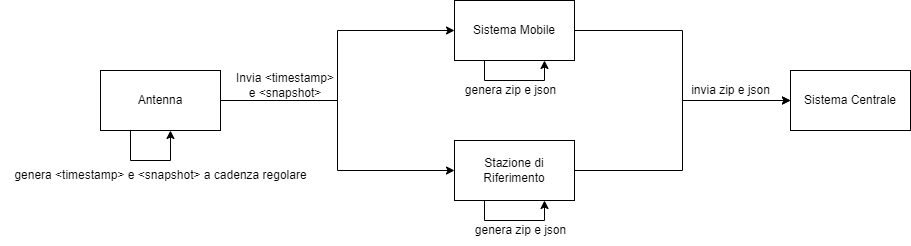
\includegraphics[scale=0.5]{images/ricezione_snapshot.png}
\caption{Un esempio di funzionamento della componente antenna per la ricezione degli snapshot}
\label{fig: ricevi_snapshot }
\end{figure}

\section{Sviluppo dello smart contract}
Gli smart contract in generale sono programmi che vengono archiviati sulla blockchain ed eseguiti quando vengono soddisfatte determinate condizioni; possono generare transazioni di pagamenti, asset e memorizzare valori sulla blockchain e l’archiviazione su questi contratti può essere globale\footnote{L’archiviazione globale è formata dai dati che vengono specificatamente memorizzati sulla blockchain a livello globale.} o locale\footnote{Le variabili locali vengono archiviate nell'account che ha aderito allo smart contract con la fase di opt-in.}. Nella fase di creazione dello smart contract è necessario specificare il numero massimo di variabili locali e globali poiché questi valori non potranno più essere modificati. Lo smart contract implementato è stato allocato con una variabile locale \textit{hash\_snapshot\_sm} e una globale chiamata \textit{Address Sistema Centrale}, entrambe di tipo byteslice (stringa di byte). La variabile globale contiene l'indirizzo pubblico dell'account Algorand del sistema centrale e viene fornita la possibilità di poterla modificare sfruttando il metodo dello smart contract \textit{set\_sistema\_centrale}. Questa variabile globale assicura che i metodi dello smart contract del sistema centrale possano essere effettivamente eseguiti solo dall'account Algorand di quest'ultimo. Infatti, i metodi (\textit{compare\_hash} e \textit{validate\_snapshot}), una volta chiamati, controllano che l'indirizzo del mittente della transazione sia uguale al valore della variabile globale \textit{Address Sistema Centrale}. Questo controllo, certifica che la chiamata di questi due metodi sia un'esclusiva del sistema centrale evitando che chiunque possa richiamarli senza permesso. La variabile locale invece è associata all'account che fa opt-in con lo smart contract creato. Di conseguenza, nel nostro caso, facendo opt-in viene allocato uno spazio di memoria sull'account Algorand per la memorizzazione della variabile locale. Al primo avvio del sistema centrale si effettua una transazione di tipo opt-in per verificare che l'account Algorand di quest'ultimo sia collegato allo smart contract. Per chiarire l'argomento, mostriamo i metodi dello smart contract che abbiamo implementato:
\begin{itemize}
    \item set\_sistema\_centrale: metodo utile nel caso ci sia bisogno di revocare i diritti ad un sistema centrale a favore di un altro. Può essere chiamato solo dall’Account Intecs.
    \item insert\_local\_hash: metodo che prende come argomento una stringa che rappresenta l'hash dello snapshot ricevuto da antenna e lo inserisce nella variabile locale hash\_snapshot\_sm associata all'account Algorand del sistema mobile. Può essere chiamato solo dal sistema mobile. L'hash dello snapshot si calcola applicando la funzione hash sha\_256 \cite{gilbert2003security} direttamente allo snapshot cioè alla stringa ricevuta da antenna.
    \item compare\_hash: metodo utilizzato dall’account sistema centrale per confrontare due byteslice. Confronta la variabile locale di Account sistema mobile con il primo argomento passato hash(snapshot\_sm).
    \item validate\_snapshot: metodo chiamato dall’account sistema centrale che inserisce in blockchain lo snapshot validato.
\end{itemize}


\subsection{Variabile locale dello smart contract}
Con l'operazione di opt-in del sistema mobile allo smart contract, l'account aderisce a quest'ultimo e nel suo account viene allocato lo spazio per le variabili locali nel caso queste siano state specificate nella fase di creazione dello smart contract. Nella figura \ref{fig: statolocale}, mostriamo la chiamata \textit{hash\_snapshot\_sm} attraverso il quale viene assegnato il valore alla variabile \textit{insert\_local\_hash}.

\begin{figure}[!h]
\centering
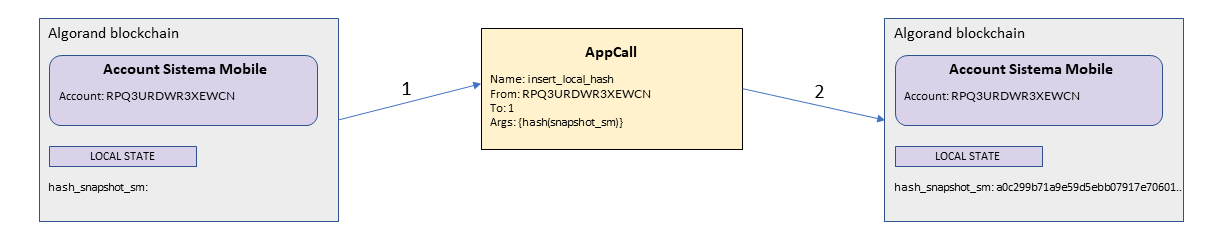
\includegraphics[scale=0.5]{images/local_state.png}
\caption{Un esempio di assegnamento ad una variabile locale}
\label{fig: statolocale}
\end{figure}

\subsection{Gestione degli account Algorand}
Per inviare qualsiasi tipo di transazione, creare smart contract e richiamare i metodi di quest'ultimo è necessario possedere un account Algorand. Poiché nel progetto è stata sfruttata la rete Testnet, gli account vengono creati su questa rete. Il codice per creare un account Algorand sfruttando Python è molto semplice:
\begin{pythoncode}
import json
from algosdk import account, mnemonic

acct = account.generate_account()
address1 = acct[1]
print("Account 1")
print(address1)
mnemonic1 = mnemonic.from_private_key(acct[0])
print("mnemonic1 = \"{}\"".format(mnemonic1))

# l'output del terminale sarà simile a:
# Account 1
# KECA5Z2ZILJOH2ZG7OPKJ5KMFXP5XBAOC7H36TLPJOQI3KB5UIYUD5XTZU
# mnemonic1 = "consider round clerk soldier hurt dynamic floor video
# output spoon deliver virtual zoo inspire rubber doll nose warfare 
# improve abstract recall choice size above actor"
\end{pythoncode}
La creazione dell'account restituisce una chiave pubblica e una privata. La pubblica è visibile a tutti mentre la privata va mantenuta nascosta agli altri utenti di Algorand. Quando si vuole inviare una transazione, la chiave pubblica diventa utile per creare la transazione non firmata. La privata invece si utilizza per firmare la transazione, un passo fondamentale per evitare che chiunque possa effettuare transazioni con account di altri utenti. La blockchain di Algorand supporta anche le chiavi mnemoniche che vengono generate durante la registrazione dell'account. Una chiave mnemonica è un modello di 25 parole che rappresenta al meglio la chiave privata ed esegue le stesse funzioni di quest'ultima. Una volta creato l'account, il suo Wallet deve essere ricaricato con Algos, la moneta della Testnet e l'operazione avviene sfruttando l'Algorand Dispenser. E' sufficiente utilizzare la chiave pubblica dell'account Algorand per poter ricaricare il Wallet associato [vedi figura \ref{fig: dispenseralgorand}].
\begin{figure}[!h]
\centering
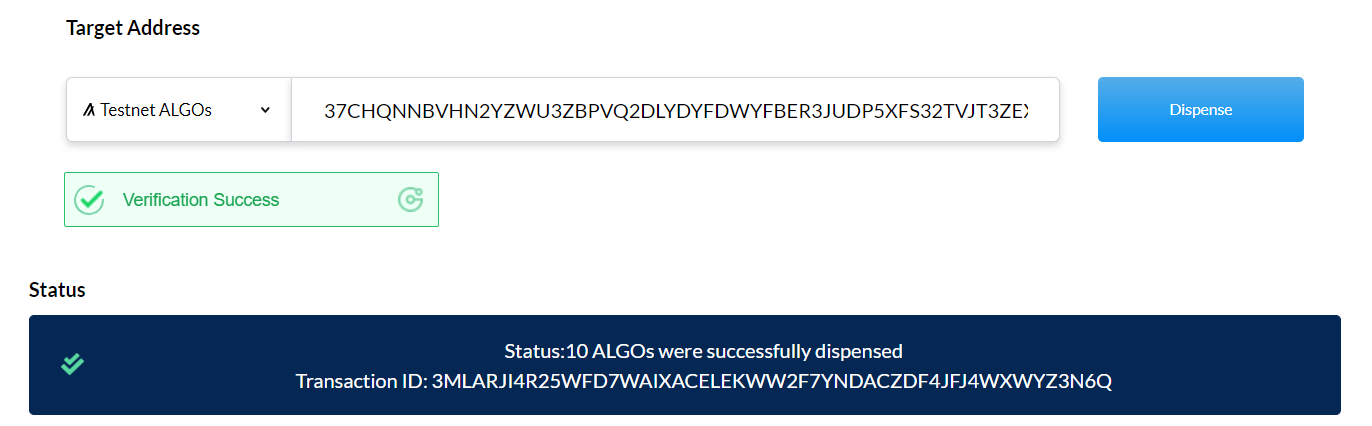
\includegraphics[scale=0.5]{images/algorand_dispenser.png}
\caption{Un esempio di utilizzo del Dispenser di Algorand}
\label{fig: dispenseralgorand}
\end{figure}
Questo tipo di operazione deve essere effettuata per creare l'account Intecs, utilizzato per creare, gestire e poter chiamare il metodo \textit{set\_sistema\_centrale} dello smart contract. Si crea anche l'account associato al sistema centrale che ci servirà per chiamare i metodi \textit{compare\_hash} e \textit{validate\_snapshot}. Infine è necessario un account Algorand per ogni sistema mobile funzionante, per poter richiamare il metodo \textit{insert\_local\_hash} dello smart contract. La stazione di riferimento e l'antenna non interagiscono con la blockchain e lo smart contract creato, non necessitano quindi di un Algorand account.
Di seguito vediamo anche un esempio completo che illustra come inviare rapidamente una semplice transazione:
\begin{pythoncode}
import json
import base64
from algosdk import account, mnemonic, constants
from algosdk.v2client import algod
from algosdk.future import transaction


def generate_algorand_keypair():
    private_key, address = account.generate_account()
    print("My address: {}".format(address))
    print("My private key: {}".format(private_key))
    print("My passphrase: {}".format(mnemonic.from_private_key(private_key)))

# Write down the address, private key, and the passphrase for later usage
generate_algorand_keypair()

def first_transaction_example(private_key, my_address):
    algod_address = "http://localhost:4001"
    algod_token = 64 * "a"
    algod_client = algod.AlgodClient(algod_token, algod_address)

    print("My address: {}".format(my_address))
    account_info = algod_client.account_info(my_address)
    print("Account balance: {} microAlgos".format(account_info.get('amount')))

    # build transaction
    params = algod_client.suggested_params()
    # comment out the next two (2) lines to use suggested fees
    params.flat_fee = constants.MIN_TXN_FEE 
    params.fee = 1000
    receiver = "HZ57J3K46JIJXILONBBZOHX6BKPXEM2VVXNRFSUED6DKFD5ZD24PMJ3MVA"
    amount = 100000
    note = "Hello World".encode()

    unsigned_txn = transaction.PaymentTxn(my_address, params, receiver, amount, 
    None, note)

    # sign transaction
    signed_txn = unsigned_txn.sign(private_key)

    # submit transaction
    txid = algod_client.send_transaction(signed_txn)
    print("Signed transaction with txID: {}".format(txid))

    # wait for confirmation 
    try:
        confirmed_txn = transaction.wait_for_confirmation(algod_client, txid, 4)  
    except Exception as err:
        print(err)
        return

    print("Transaction information: {}".format(
        json.dumps(confirmed_txn, indent=4)))
    print("Decoded note: {}".format(base64.b64decode(
        confirmed_txn["txn"]["txn"]["note"]).decode()))

    print("Starting Account balance: {} microAlgos".format(account_info.get
    ('amount')) )
    print("Amount transfered: {} microAlgos".format(amount) )    
    print("Fee: {} microAlgos".format(params.fee) ) 


    account_info = algod_client.account_info(my_address)
    print("Final Account balance: {} microAlgos".format(account_info.get
    ('amount')) + "\n")

# replace private_key and my_address with your private key and your address.
first_transaction_example(private_key, my_address)
\end{pythoncode}

\subsection{Principio di funzionamento generale}
Vediamo di seguito, attraverso una rappresentazione grafica [vedi figura \ref{fig: architetturasistema }], il funzionamento del nuovo sistema realizzato che introduce la tecnologia blockchain. Nella figura per semplicità, non sono state inserite le frecce di conferma transazione del metodo dello smart contract insert\_local\_hash e di compare\_hash.

\begin{figure}[!h]
\centering
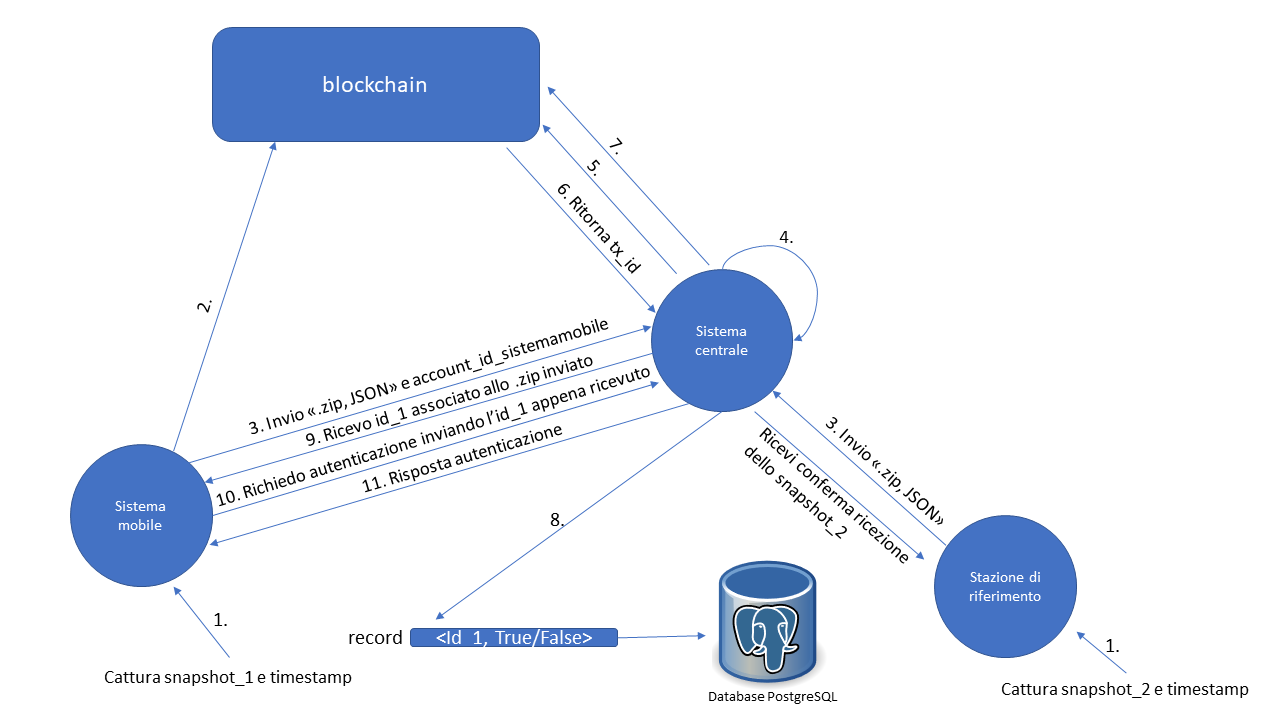
\includegraphics[scale=0.5]{images/schema progetto con blockchain v2.png}
\caption{Architettura del nuovo sistema}
\label{fig: architetturasistema }
\end{figure}

\begin{itemize}
\item 1: la componente antenna invia lo snapshot\_1 al sistema mobile e lo snapshot\_2 alla stazione di riferimento insieme al timestamp (sia lo snapshot che il timestamp sono uguali per entrambi).
\item 2: il sistema mobile invoca il metodo \textit{insert\_local\_hash} dello smart contract passandogli come argomento l'hash dello snapshot\_1 ricevuto da antenna. Il risultato del passo 2 è che l'account Algorand di sistema mobile scrive sulla propria variabile locale hash\_snapshot\_sm il risultato della funzione hash sha\_256 applicata a snapshot\_1.
\item 3: dopo aver acquisito lo snapshot e il timestamp da antenna, il sistema mobile memorizza lo snapshot in un file all'interno di un archivio zip, genera le informazioni di posizione e insieme al timestamp le inserisce in un file JSON per poi inviarle al sistema centrale assieme al proprio indirizzo Algorand (chiave pubblica). Anche la stazione di riferimento, eseguendo le medesime procedure, invierà un file zip e un file JSON.
\item 4: il sistema centrale confronta lo snapshot ricevuto al passo 3 dal sistema mobile e dalla stazione di riferimento.
\item 5: il sistema centrale dopo aver verificato l'uguaglianza degli snapshot al passo 4 può chiamare il metodo dello smart contract \textit{compare\_hash} con i seguenti parametri:
\begin{itemize}
    \item hash(snapshot\_1): lo calcola sfruttando lo snapshot\_1 ottenuto al passo 3.
    \item account\_id\_sistemamobile: lo ottiene al passo 3 e gli serve per accedere alla variabile locale di sistema mobile per acquisire l’hash\_snapshot\_sm e confrontarlo con il primo parametro passato.
\end{itemize}
In pratica lo smart contract valida lo snapshot\_1 controllando che non sia stato alterato al passo 3.
\item 6: se la verifica che lo snapshot\_1 non sia stato alterato al passo 3 è andata a buon fine, viene restituita la transaction\_id (tx\_id) della transazione effettuata al passo 5.
\item 7: non appena il sistema centrale riceve al passo 6 la tx\_id è sicuro che lo snapshot\_1 non sia stato alterato. E' possibile quindi far confrontare lo snapshot\_1 (ricevuto dal sistema mobile) con lo snapshot\_2 (ricevuto dalla stazione di riferimento) al sistema centrale, ed inviare poi, nel caso l'operazione vada a buon fine, una transazione di conferma validazione alla blockchain sfruttando il metodo \textit{validate\_snapshot} dello smart contract che conterrà le seguenti informazioni nel campo nota:
\begin{itemize}
    \item l'id dello snapshot
    \item l'hash dello snapshot del sistema mobile
    \item l'account address del sistema mobile
    \item il timestamp
    \item i dati di posizione dello snapshot certificato (latitudine, longitudine, altitudine)
\end{itemize}
\item 8: al passo 8 viene salvato in un database PostgreSQL interno al sistema centrale il record <id\_1, True/False> dove: l’id\_1 rappresenta l’identificatore univoco del file zip ricevuto da sistema mobile e il secondo campo contiene un booleano che è impostato a True se lo snapshot ricevuto dal sistema mobile non è stato alterato, False altrimenti. Questo meccanismo consente al sistema mobile di poter richiedere l’autenticazione dell’id dello snapshot al sistema centrale quando vuole senza necessità che quest'ultimo ogni volta effettui nuovamente le varie operazioni di confronto tra snapshot.
\item 9: al passo 9 il sistema centrale invia l'id che aveva precedentemente associato allo snapshot (file binario) ricevuto dal sistema mobile a quest'ultimo.
\item 10: il sistema mobile attraverso l'interfaccia a linea di comando cli può richiedere in ogni momento le informazioni di autenticazione dello snapshot tramite l'id ricevuto al passo 8.
\item 11: il sistema centrale invia l’esito dell'autenticazione della posizione al sistema mobile che può essere positivo e in quel caso significa che la posizione è stata autenticata correttamente, altrimenti significa che lo snapshot ricevuto dal sistema mobile è stato corrotto.
\end{itemize}

\subsection{Interazione con la Blockchain}
Il diagramma di sequenza in figura \ref{fig: diagramactivity1} mostra chiaramente le varie interazioni con la blockchain e più nel dettaglio le chiamate che vengono effettuate allo smart contract. Nel progetto di base, il sistema mobile e la stazione di riferimento sono sincronizzati con un orologio atomico che a cadenza regolare di 120 secondi calcola un timestamp \footnote{Un timestamp è una sequenza di caratteri che rappresentano una data e/o un orario per accertare l'effettivo avvenimento di un certo evento.} e inizia a registrare il segnale proveniente dai satelliti Galileo per circa 5 secondi. Questa procedura viene simulata tramite l'invio da parte del sistema antenna di un timestamp e di uno snapshot rispettivamente al sistema mobile e alla stazione di riferimento a cadenza di 120 secondi. Il compito del sistema mobile a questo punto sarà quello di costruire il file zip con all'interno il file snapshot.bin che contiene lo snapshot ricevuto poco fa. 
\begin{figure}[!h]
\centering
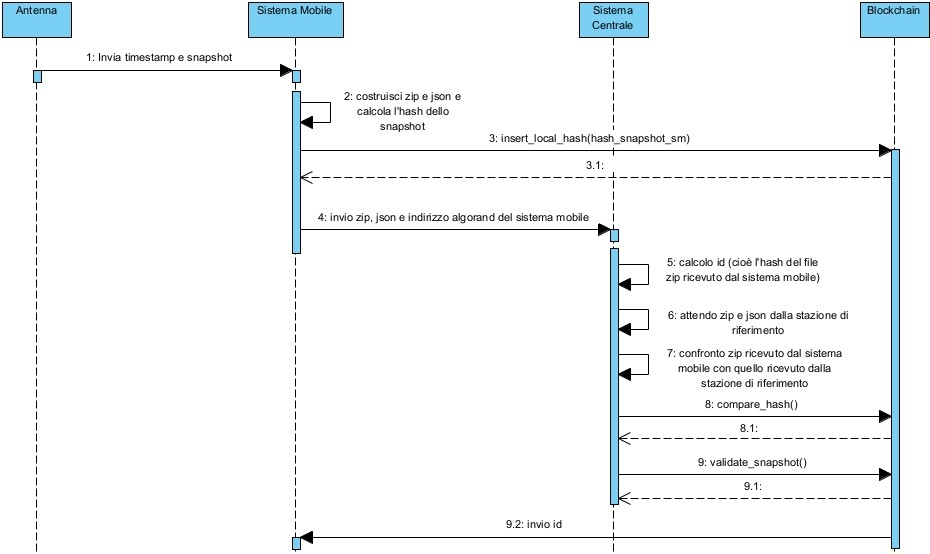
\includegraphics[scale=0.6]{images/Sequence Diagram - scambio msg con blockchain.jpg}
\caption{Diagramma di sequenza dell'interazione con lo smart contract}
\label{fig: diagramactivity1}
\end{figure}\\
Il sistema mobile costruisce anche il file json dei metadati a partire dal timestamp e avrà la seguente forma:\\
\lstinputlisting[label= cod: metadati, caption= esempio di dati di posizione contenuti nel file json dei metadati, language=json, basicstyle=\small]{listing/sourceCode/metadati.json}
Dove i parametri di latitudine, longitudine e altitudine vengono generati casualmente. Lo snapshot reale e cioè quello catturato dai satelliti Galileo, contiene molti altri parametri, ma visto che si tratta di una simulazione solo a scopo di progetto, quelli utilizzati sono sufficienti. Sfruttando la funzione sha\_256 è possibile calcolare l'hash dello snapshot semplicemente applicandola a snapshot.bin che si trova all'interno del file zip generato. E' a questo punto che viene chiamato il metodo dello smart contract \textit{insert\_local\_hash} il cui argomento passato è l'hash dello snapshot appena calcolato. Il sistema mobile invierà i due file zip, json e il proprio indirizzo Algorand al sistema centrale, il quale calcolerà l'id dello snapshot appena ottenuto tramite il calcolo dell'hash del file zip del sistema mobile. Quando il sistema centrale è sicuro di aver ricevuto il file zip e json anche dalla stazione di riferimento può confrontare lo zip del sistema mobile con quello ricevuto dalla stazione di riferimento e chiamare il metodo \textit{compare\_hash} con i seguenti argomenti: hash(snapshot\_1) che lo calcola sfruttando lo snapshot\_1 ottenuto al passo 3 e l'account\_id\_sistemamobile  (anche questo ottenuto al passo 3) che utilizza per accedere alla var. locale di sistema mobile per acquisire l’hash\_snapshot\_sm e confrontarlo con il primo argomento passato. Questa operazione accerta che lo snapshot ottenuto dal sistema mobile non sia stato alterato nell'invio. Se anche questo metodo è andato a buon fine si può certificare lo snapshot di partenza attraverso la chiamata di \textit{validate\_snapshot} e registrare la posizione in blockchain, rendendola di fatto, immutabile.

\section{Sistema Centrale}
Il sistema centrale rappresenta il modulo più importante perché svolge molteplici compiti. Esso infatti, comunica sia con il sistema mobile che con la stazione di riferimento per ottenere i file zip e JSON degli snapshot. Ne effettua anche il salvataggio per poi essere in grado di poterli confrontare ed eventualmente certificare la posizione.
A livello di comunicazione sono stati implementati tre server TCP, ognuno gestito da un diverso thread in continuo ascolto. Elenchiamo di seguito i tre server:
\begin{itemize}
    \item server\_sm: server TCP che comunica con il sistema mobile per la ricezione dei file zip e JSON. Rimane in ascolto di nuove connessioni da parte del sistema mobile e non appena ne arriva una, avvia il thread "thread\_sm" per gestirla.
    \item server\_sr: server TCP che comunica con la stazione di riferimento per la ricezione dei file JSON e zip. Rimane in ascolto di nuove connessioni da  parte dei sistemi mobile e non appena ne arriva una, avvia il thread "thread\_sr" per gestirla.
    \item server\_sm\_cli: server TCP che comunica con il sistema mobile per la ricezione degli id, l'invio dell'esito dell'autenticazione dello snapshot e della lista di tutti gli id ricevuti alla cli. Rimane in ascolto di nuove connessioni da parte dei sistemi mobile. Non appena si avvia un sistema mobile, questo si collegherà in automatico al server. Infatti, il server avvierà un thread "thread\_sm\_cli" che gestirà autonomamente la comunicazione con quel sistema mobile.
\end{itemize}
Ciascuno di questi server quindi, non appena riceve una richiesta dal sistema mobile o dalla stazione di riferimento per aprire una nuova comunicazione, avvierà un thread per la gestione della connessione.

\subsection{File di configurazione}
Nella cartella di sistema\_centrale si trova anche il file info\_algorand.json che contiene i parametri fondamentali per potersi collegare alla blockchain e allo smart contract. 
\lstinputlisting[label= cod: request, caption= esempio del contenuto nel file info\_algorand.json, language=json, basicstyle=\small]{listing/sourceCode/info_algorand.json}

In sintesi, contiene i campi dell'account Algorand del sistema centrale e l'id della dApp creata da Intecs.

\subsection{Persistenza dei dati}
\subsubsection{Database PostgreSQL}
Il sistema centrale memorizza gli id degli snapshot insieme all'esito dell'autenticazione di questi. L'id si ottiene calcolando l'hash del file zip ricevuto dal sistema mobile mentre l'esito dipenderà dal confronto dello snapshot contenuto dal file zip con quello ricevuto dalla stazione di riferimento. Il valore di esito sarà un valore booleano True o False. Il record <id, esito> verrà a questo punto inserito nel database di tipo PostgreSQL e servirà al sistema centrale nel momento in cui il sistema mobile effettuerà una richiesta di autenticazione dello snapshot. Il sistema centrale memorizza poi gli snapshot e i metadati in due database (object storage e database metadati).

\subsubsection{Salvataggio dei file zip e JSON}
Il sistema centrale come sappiamo riceve a intervalli regolari coppie di zip e JSON dai sistemi mobili e dalle stazioni di riferimento e quest'ultimi vengono memorizzati. Per mapparli correttamente vengono mantenuti aggiornati due file all'interno della directory che contiene anche i file zip e JSON. Essi sono:
\begin{itemize}
    \item object\_storage: è un file JSON che contiene le coppie <id,path> dei file zip
    \item metadati.json: è un file JSON che contiene le coppie <id,path> dei file JSON
\end{itemize}

\section{Sistema Mobile}
Il sistema mobile rimane in ascolto degli snapshot da antenna. Come già detto in precedenza, riceve un timestamp e uno snapshot a cadenza regolare e comunica con il sistema centrale tramite connessione TCP per l'invio dei file zip e JSON degli snapshot. Ha un ruolo da intermediario tra la Cli\footnote{La Cli è un programma implementato con un'interfaccia a linea di comando utilizzato per poter richiedere informazioni sugli snapshot e sarà introdotto nel capitolo \ref{5.cli e intecs}.} e il sistema centrale, ma questo lo approfondiremo meglio nel capitolo \ref{capitolo_cli}.

\subsection{File di configurazione}
Nella cartella di sistema\_mobile dove si trova il file sistemamobile.py è presente anche il file di configurazione info\_algorand.json che contiene l'indirizzo dell'account Algorand del sistema mobile e l'id dell'applicazione creata da Intecs SpA. 
\lstinputlisting[label= cod: metadati1, caption= esempio del contenuto nel file info\_algorand.json, language=json, basicstyle=\small]{listing/sourceCode/info_algorand_sm.json}

\subsection{Salvataggio dei dati}
Viene mantenuto un file chiamato id\_list di tipo JSON che su ogni riga contiene alcune informazioni riferite ad un particolare id, ciascuna informazione è delimitata da uno spazio dove la prima informazione rappresenta l'identificatore dello snapshot. Il calcolo dell'identificatore (id) si ottiene applicando la funzione sha\_256 a 'snapshot.bin' all'interno del file zip ricevuto dal sistema mobile. Le due informazioni successive rappresentano rispettivamente la data e l'ora di ricezione dell'identificatore. L'ultimo parametro invece rappresenta un valore booleano che vale True se la certificazione della posizione è avvenuta correttamente e vale False altrimenti [vedi figura \ref{fig: record_id_list }].

\begin{figure}[!h]
\centering
\includegraphics[scale=0.8]{images/record id\_list.png}
\caption{Un esempio di record di id\_list}
\label{fig: record_id_list }
\end{figure}

\section{Stazione di Riferimento}
Come per il sistema mobile anche questa componente rimane in ascolto di timestamp e snapshot dalla componente antenna e comunica con il sistema centrale tramite connessione TCP per l’invio dei file zip e JSON degli snapshot.

\section{Struttura delle cartelle e dei file del progetto}
La cartella \textbf{antenna} contiene i seguenti file:
\begin{itemize}
    \item Dockerfile
    \item config.json
\end{itemize}
La cartella \textbf{intecs} contiene i seguenti file:
\begin{itemize} 
    \item intecs.py 
    \item config.json 
\end{itemize}
La cartella \textbf{sistema\_mobile} contiene i seguenti file e cartelle:
\begin{itemize}
    \item sistemamobile.py 
    \item Dockerfile 
    \item utility.py 
    \item info\_algorand.json
    \item \textbf{cli}
        \begin{itemize}
            \item cli.py
            \item Dockerfile
        \end{itemize}
    \item \textbf{cli v2}
        \begin{itemize}
            \item cli.py 
            \item config.json 
        \end{itemize}
\end{itemize}
La cartella \textbf{sistema\_centrale} contiene i seguenti file:
\begin{itemize}
    \item sistemacentrale.py 
    \item database\_library.py 
    \item Dockerfile 
    \item utility.py 
    \item info\_algorand.json 
\end{itemize}
La cartella \textbf{stazione\_di\_riferimento} contiene i seguenti file:
\begin{itemize}
    \item stazioneriferimento.py 
    \item Dockerfile 
    \item utility.py 
\end{itemize}

\section{Docker}
Il nuovo sistema di certificazione della posizione è stato sviluppato sfruttando Docker Desktop su ambiente Windows. Per far funzionare il progetto con Docker è necessario aver installato sul proprio computer Docker e Docker Compose \cite{dockerinstall}.

\subsection{Avvio del progetto}
E' possibile avviare il progetto di simulazione lanciando il comando \textit{docker-compose up} dalla cartella principale che contiene il file docker-compose.yml.

\subsection{Struttura dei container}
I container di cui si fa uso nel progetto di simulazione sono cinque: 
\begin{itemize}
    \item il sistema centrale
    \item il sistema mobile
    \item la stazione di riferimento
    \item la cli
    \item il database Postgres
\end{itemize}

\subsection{Ordine di avvio}
L'ordine di avvio dei container è il seguente:
\begin{enumerate}
    \item database Postgres
    \item sistema centrale
    \item sistema mobile
    \item cli
    \item stazione di riferimento
\end{enumerate}

\section{Cli - Avvio con Docker Desktop}
Se il progetto è stato eseguito con docker-compose e vogliamo avviare il programma Cli è necessario utilizzare Docker Desktop. Assicurandosi di aver avviato il progetto con il comando \textit{docker-compose up} dalla cartella principale del progetto che contiene il file docker-compose.yml, possiamo procedere all'avvio della Cli. Selezioniamo dalla lista dei container del progetto il container riferito alla Cli e clicchiamo sull'icona del terminale CLI [vedi figura \ref{fig: docker_2 }].
\begin{figure}[!h]
\centering
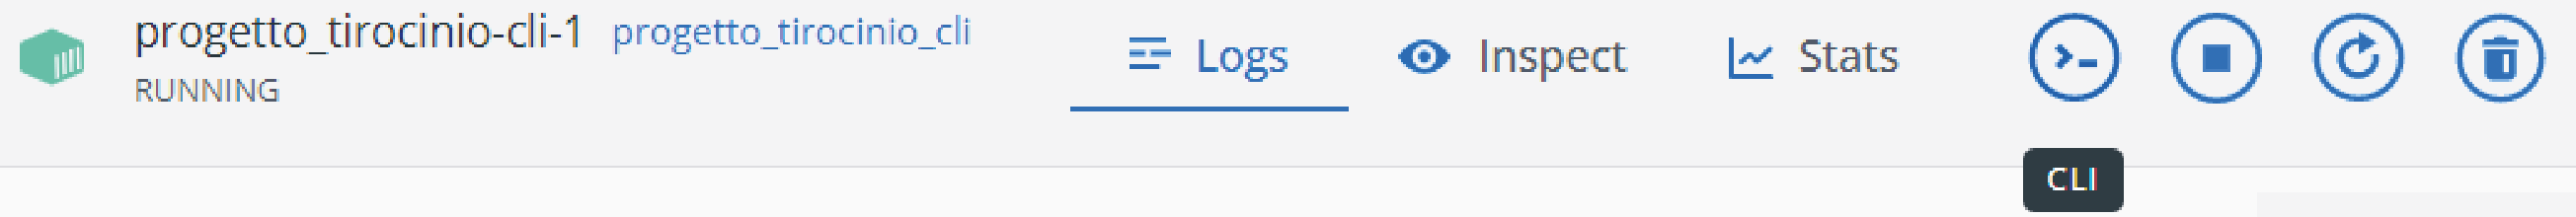
\includegraphics[scale=0.7]{images/docker_2.png}
\caption{Schermata che mostra il pulsante del terminale CLI}
\label{fig: docker_2 }
\end{figure}\\
E' sufficiente, arrivati a questo punto, eseguire dalla console appena aperta il comando \textit{python cli.py} per avviare il programma Cli, come nella figura \ref{fig: docker_3 }.
\begin{figure}[h]
\centering
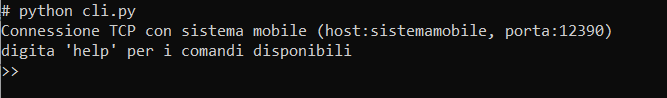
\includegraphics[scale=0.9]{images/docker_3.png}
\caption{Avvio della Cli da Docker Desktop}
\label{fig: docker_3 }
\end{figure}


\chapter{Cli e Intecs}\label{5.cli e intecs}
In questo capitolo introdurremo due programmi fondamentali implementati con un'interfaccia a linea di comando, entrambi sviluppati con Python, che ci daranno la possibilità di interagire con il progetto realizzato.

\section{Cli}\label{capitolo_cli}
L'interfaccia a linea di comando Cli è uno strumento utile per poter richiedere informazioni sugli snapshot attraverso gli id forniti dal sistema centrale. Il codice del programma è presente al percorso \textit{sistema\_mobile/cli} nel file cli.py. Ogni sistema mobile avviato ha a disposizione un programma che gestisce un'interfaccia a linea di comando chiamata Cli attraverso il quale è possibile interfacciarsi al sistema mobile per poterlo interrogare. L'architettura del programma Cli è molto semplice: è stata implementata una connessione tra il sistema mobile e la Cli e tra il sistema mobile e il sistema centrale, sfruttando per entrambe le connessioni il protocollo TCP.

\subsection{Configurazione tra Cli e Sistema Mobile}
Per avviare correttamente il nuovo sistema di certificazione realizzato, è necessario configurare la comunicazione TCP tra la componente sistema mobile e il programma Cli. Operazione realizzata attraverso la semplice modifica di due variabili presenti sia nel file Python sistemamobile.py, contenuto nella cartella \textit{sistema\_mobile} che nel file cli.py, contenuto nel percorso \textit{sistema\_mobile/cli}. Per comodità, le due variabili presenti nei due file assumono lo stesso nome: host\_cli e port\_cli. E' doveroso ribadire anche se evidente, che la variabile host\_cli oltre a contenere un indirizzo host valido dovrà apparire con lo stesso valore in entrambi i file e la stessa considerazione varrà anche per port\_cli anche se in questa circostanza dovrà invece contenere un numero di porta valido.
\subsection{Autenticazione degli id}\label{autenticazionedegliid}
\begin{figure}[!h]
\centering
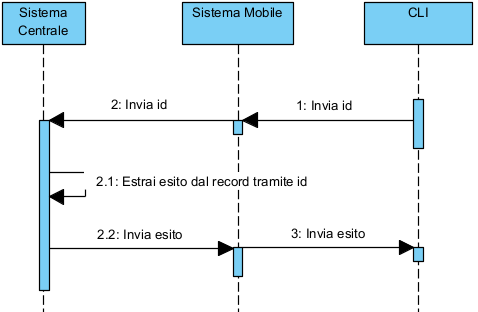
\includegraphics[scale=0.9]{images/Richiesta autenticazione id.png}
\caption{Richiesta autenticazione di un id}
\label{fig: richiesta_autenticazione_id }
\end{figure}
Il sistema centrale come già sappiamo, confronta lo snapshot ricevuto dal sistema mobile con quello ricevuto dalla stazione di riferimento, calcola l'identificatore (o id) associato allo snapshot ricevuto dal sistema mobile sfruttando una funzione hash\footnote{La funzione hash utilizzata è la sha\_256 e viene applicata allo snapshot ricevuto dal sistema mobile.}, e infine lo invia a quest'ultimo. E' attraverso questo id che il sistema mobile può richiedere l'esito dell'autenticazione dello snapshot oltre ad altre informazioni. Per richiedere l'autenticazione degli id si sfrutta il comando \textit{verifica\_id <id>}. L'implementazione avviene con una comunicazione TCP tra la Cli e il sistema mobile che a sua volta comunicherà con il sistema centrale, il quale ci restituirà un valore booleano [vedi figura \ref{fig: richiesta_autenticazione_id }]. Il valore booleano restituito sarà True se l'id associato allo snapshot è stato autenticato correttamente, False altrimenti. Una risposta negativa ci fa intendere che lo snapshot associato all'id da verificare è stato corrotto. Qualche malintenzionato ha quindi interferito con il ricevitore satellitare del sistema mobile facendo sì che il segnale non fosse catturato dai satelliti, ma da un terzo dispositivo che inviava dati manipolati. In figura \ref{fig: verifica_id } mostriamo un esempio di utilizzo del comando \textit{verifica\_id}.
\begin{figure}[!h]
\centering
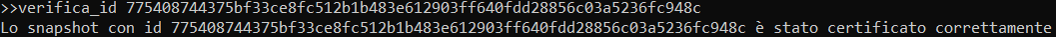
\includegraphics[scale=0.8]{images/verifica_id.png}
\caption{Un esempio di utilizzo del comando verifica\_id}
\label{fig: verifica_id }
\end{figure}

\subsection{Stampa lista degli id}
Attraverso il comando \textit{stampa\_lista\_id} è possibile richiedere tutti gli id inviati dal sistema centrale al sistema mobile fino a quel momento. Ogni volta che il sistema mobile riceve un id dal sistema centrale lo memorizza all'interno del file id\_list.json, in questo modo manterrò la persistenza degli id e quando dal programma Cli voglio ottenerli, sarà sufficiente inviare una richiesta al sistema mobile che inoltrerà l'intera lista. Nella figura \ref{fig: stampalistaid } mostriamo un esempio di utilizzo del comando.
\begin{figure}[!h]
\centering
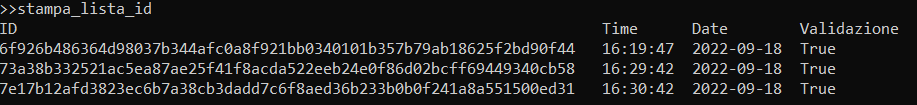
\includegraphics[scale=0.8]{images/stampa_lista_id.png}
\caption{Un esempio di utilizzo del comando stampa\_lista\_id}
\label{fig: stampalistaid }
\end{figure}

\subsection{Info posizione a partire da un id}
La procedura di richiesta delle informazioni di posizione a partire da un id, avviene con il comando \textit{info\_id <id>}, che si comporta in maniera molto simile alla procedura di richiesta dell'esito dell'autenticazione degli snapshot vista sopra [vedi sottosezione \ref{autenticazionedegliid}]. Il primo messaggio viene inviato dalla Cli e rappresenta una stringa che contiene il comando "info\_id", per far capire al sistema mobile il tipo di operazione da svolgere. Ricevuta la conferma di ricezione del messaggio può inviare l'id da verificare. Il sistema mobile, dopo aver ricevuto questi due messaggi può comunicare con il sistema centrale, il quale, dopo aver ricevuto l'id sfrutta il file metadati.json. In tal modo ottiene il file dei metadati associato a quell'identificatore (id) per estrarre le informazioni di posizione da inviare al sistema mobile per poi essere inoltrate alla Cli. Per chiarire meglio le idee è possibile visionare il diagramma di sequenza in figura \ref{fig: informazioni_id } che spiega lo scambio di messaggi step by step. Nella figura \ref{fig: info_id2 } vediamo invece un esempio di utilizzo del comando \textit{info\_id}.
\begin{figure}[!h]
\centering
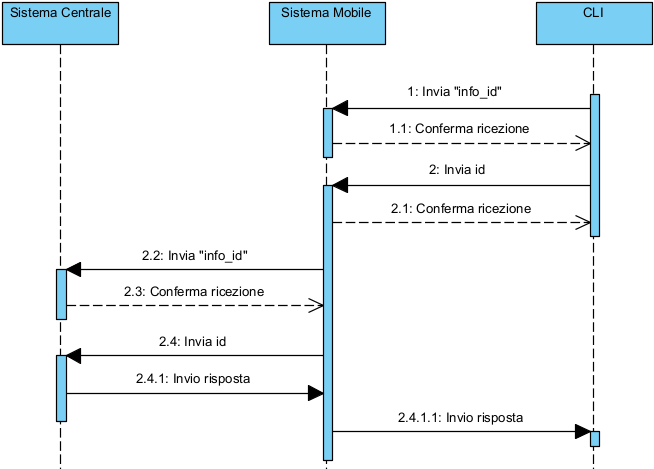
\includegraphics[scale=0.8]{images/info_id.png}
\caption{Diagramma per descrivere la comunicazione tra componenti per la realizzazione del comando info\_id}
\label{fig: informazioni_id }
\end{figure}
\begin{figure}[!h]
\centering
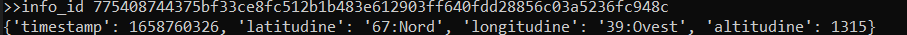
\includegraphics[scale=0.8]{images/info_id2.png}
\caption{Un esempio di utilizzo del comando info\_id}
\label{fig: info_id2 }
\end{figure}

\subsection{Altri comandi}
Vediamo gli altri comandi disponibili con l'interfaccia a linea di comando Intecs.
\begin{itemize}
    \item \textit{help}: restituisce la lista di tutti i comandi disponibili con una piccola didascalia per rendere più chiaro il funzionamento di ognuno di questi.
    \item \textit{clear}: ripulisce la schermata del programma cancellando ogni scritta presente.
    \item \textit{exit}: viene usato per chiudere correttamente il programma.
\end{itemize}

\subsection{Tabella riassuntiva dei comandi}
\scalebox{0.9}{
\begin{tabular}{llllll}
\toprule
{\bfseries Comando} & {\bfseries Sintassi} & {\bfseries
Esempio}\\
\midrule
stampa\_lista\_id & stampa\_lista\_id  & stampa\_lista\_id \\
\midrule
verifica\_id & verifica\_id <id> & verifica\_id 597c28c381ef1fee \\
\midrule
info\_id & info\_id <id> & info\_id 597c28c381ef1fee \\
\midrule
help & help & help \\
\midrule
exit & exit & exit \\
\midrule
clear & clear & clear \\
\bottomrule
\end{tabular}}

% \hspace{-1.7 cm}
% \begin{center}
% \centering
% \begin{tabular}{|l|c|c|}
% \hline
% \multicolumn{3}{|c|}{}\\
% \multicolumn{3}{|c|}{\textbf{\Large Comandi}}\\
% \multicolumn{3}{|c|}{}\\
% \hline
% \multicolumn{1}{|c|}{\textbf{Comando}} & \textbf{Sintassi} &
% \multicolumn{1}{c|}{\textbf{Esempio}}\\
% \hline
% stampa\_lista\_id & stampa\_lista\_id  & stampa\_lista\_id \\
% verifica\_id & verifica\_id <id> & verifica\_id 597c28c381ef1fee \\
% info\_id & info\_id <id> & info\_id 597c28c381ef1fee \\
% help & help & help \\
% exit & exit & exit \\
% clear & clear & clear \\
% \hline
% \end{tabular}
% \end{center}

\section{Cli v2}
Sono state implementate due versioni del programma Cli implementato con un'interfaccia a linea di comando. La prima versione comunica con il sistema mobile per richiedere le informazioni degli snapshot ed è stata approfondita poco fa. In questa seconda versione invece, il programma si interfaccia direttamente con la blockchain comunicando attraverso l'Indexer V2 (approfondito nel capitolo \ref{2.statoarte}). Il codice del programma è presente al percorso \textit{sistema\_mobile/'cli v2'} nel file cli.py. Prima di poter avviare questo file Python è necessario configurare il file config.json in maniera corretta. Nel codice seguente mostriamo un fac-simile del contenuto dove \textit{indirizzo pubblico} dovrà essere sostituito con il valore dell'indirizzo pubblico Algorand del sistema centrale.
\lstinputlisting[label= cod: config1cli2, caption= esempio del contenuto nel file config.json, language=json, basicstyle=\small]{listing/sourceCode/configjson_cliv2.json}
L'implementazione di questa versione del programma è molto semplice: si estraggono le transazioni dalla blockchain il cui mittente è l'indirizzo Algorand del sistema centrale attraverso il metodo \textit{search\_transaction\_by\_address(address)} fornito dall'Indexer di Algorand. Le transazioni restituite saranno quelle riferite ai metodi \textit{compare\_hash()} e \textit{validate\_snapshot()} ma visto che ci interessa il  contenuto del campo nota utilizzeremo solo le transazioni di \textit{validate\_snapshot()}. Nella figura \ref{fig: camponota } mostriamo il campo nota  di una transazione riferita al metodo \textit{validate\_snapshot()} attraverso AlgoExplorer\footnote{AlgoExplorer è una piattaforma che consente di esplorare e cercare nella blockchain di Algorand transazioni, indirizzi, statistiche, smart contract e altro ancora.} \cite{algoexplorer}. Notiamo subito, che il campo nota è formato dai seguenti parametri:
\begin{itemize}
    \item account\_address\_sistema\_mobile: ci indica quale account Algorand del sistema mobile ha ricevuto lo snapshot in questione.
    \item id: rappresenta l'identificatore (id) univoco allo snapshot restituitoci dal sistema centrale.
    \item hash\_snapshot\_sm: rappresenta l'hash calcolato con la funzione sha\_256 dello snapshot.
    \item timestamp: rappresenta la data e l'ora in cui il sistema mobile ha ricevuto lo snapshot dalla componente antenna.
    \item latitudine, longitudine, altitudine: rappresentano dati di posizione che si riferiscono alla posizione in cui si trovava il sistema mobile al momento dell'acquisizione dei segnali da antenna.
\end{itemize}
\begin{figure}[!h]
\centering
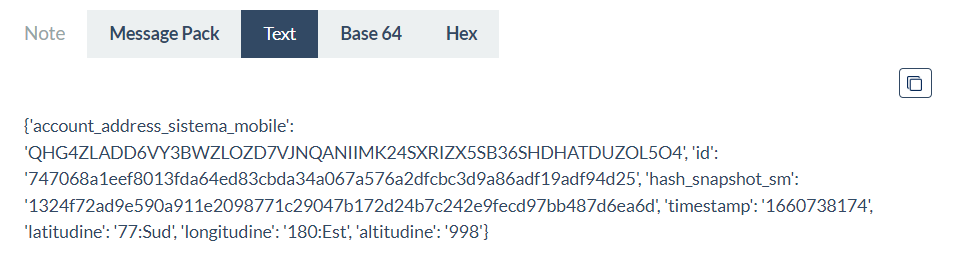
\includegraphics[scale=0.8]{images/campo_nota.png}
\caption{Un esempio del campo nota della transazione riferita al metodo validate\_snapshot()}
\label{fig: camponota }
\end{figure}
Di seguito approfondiamo l'implementazione dei comandi del programma Cli v2.

\subsection{Stampa lista degli id}\label{stampalistaid}
Il comando \textit{stampa\_lista\_id} restituisce gli id (o identificatori) inviati dal sistema centrale al sistema mobile fino a quel momento, ma non tutti, infatti ci restituisce solamente quelli il cui snapshot ha riportato un esito positivo nella certificazione. Questo per il semplice fatto che se un id associato ad uno snapshot non supera la fase di autenticazione, non sarà richiamato il metodo \textit{validate\_snapshot()} per questo snapshot e di conseguenza non compariranno in blockchain le sue informazioni. La ricerca degli id si effettua anche in questo caso, con il metodo \textit{search\_transaction\_by\_address()}, il cui argomento sarà sempre l'indirizzo Algorand del sistema centrale. Questo metodo ci restituirà una lista contenente tutte le transazioni in cui il mittente è il sistema centrale. Dovremo anche in questo caso filtrare le transazioni ed estrarre solo quelle riferite al metodo \textit{validate\_snapshot()}. Dunque, estrarremo da ognuna di queste transazioni il campo nota e da quest'ultimo acquisiremo l'id. Attraverso quest'implementazione potremo ottenere quindi, ogni id.

\subsection{Autenticazione degli id}
Il comando \textit{verifica\_id <id>} estrae la lista degli id come abbiamo visto con il comando \textit{stampa\_lista\_id} (vedi sottosezione \ref{stampalistaid}), prendendo quindi il campo id di ogni transazione e confrontandolo con il campo <id> passato per argomento. Lo scopo è di trovare la transazione il cui id corrisponde a quello passato per argomento. Se si verifica questa condizione, posso dire con certezza che lo snapshot associato a tale id è stato autenticato correttamente. Ribadiamo che gli snapshot che non superano la fase di confronto e non vengono quindi certificati, non saranno caricati sulla blockchain con la transazione riferita al metodo \textit{validate\_snapshot()}.

\subsection{Info posizione a partire da un id}
Il comando \textit{info\_id <id>} estrae il campo noto dalle transazioni riferite al metodo \textit{validate\_snapshot}, cerca la transazione il cui campo nota ha come id quello passato per argomento ed estrae i dati di posizione (latitudine, longitudine, altitudine) ed il timestamp di quel campo nota.

\subsection{Settaggio dell'indirizzo Algorand di Sistema Centrale}
Il comando \textit{set\_address\_sistemacentrale <address>} si utilizza per impostare il valore di sistema\_centrale\_address del file config.json attraverso il quale possiamo settare l'account Algorand di cui restituiremo le transazioni, tramite l'utilizzo del metodo dell'Indexer \textit{search\_transaction\_by\_address()}.

\subsection{Altri comandi}
Vediamo gli altri comandi disponibili con il programma Intecs.
\begin{itemize}
    \item \textit{help}: restituisce la lista di tutti i comandi disponibili con una piccola didascalia per rendere più chiaro il funzionamento di ognuno di questi.
    \item \textit{clear}: ripulisce la schermata del programma cancellando ogni scritta presente.
    \item \textit{exit}: viene usato per chiudere correttamente il programma.
\end{itemize}

\subsection{Tabella riassuntiva dei comandi}
\resizebox{\textwidth}{!}{%
\begin{tabular}{llllll}
\toprule
{\bfseries Comando} & {\bfseries Sintassi} & {\bfseries
Esempio}\\
\midrule
stampa\_lista\_id & stampa\_lista\_id  & stampa\_lista\_id \\
\midrule
verifica\_id & verifica\_id <id> & verifica\_id 597c28c381ef1fee \\
\midrule
info\_id & info\_id <id> & info\_id 597c28c381ef1fee \\
\midrule
set\_address\_sistemacentrale & set\_address\_sistemacentrale <address> & set\_address\_sistemacentrale 597c28c381ef1fee \\
\midrule
help & help & help \\
\midrule
exit & exit & exit \\
\midrule
clear & clear & clear \\
\bottomrule
\end{tabular}}

\section{Intecs}
Lo smart contract viene creato e gestito da Intecs SpA attraverso il programma Intecs, implementato con un'interfaccia a linea di comando per permettere alcune operazioni critiche come la creazione ed eliminazione degli smart contract. Il codice Python del programma Intecs è presente nella cartella \textit{intecs} nel file intecs.py e rappresenta proprio il programma da dover avviare per far funzionare l'interfaccia a linea di comando in questione.

\subsection{File di configurazione}
Nella cartella \textit{intecs}, oltre al file intecs.py si trova il file config.json al cui interno ha i parametri fondamentali per potersi collegare alla blockchain e allo smart contract. 
\lstinputlisting[label= cod: request, caption= esempio del contenuto nel file config.json, language=json, basicstyle=\small]{listing/sourceCode/config_intecs.json}
Contiene infatti, l'indice dello smart contract (app id) creato e l'indirizzo Algorand del sistema centrale.

\subsection{Il primo avvio del programma}
Al primo avvio del programma intecs.py viene ricordato di creare gli account Algorand, senza i quali non sarebbe possibile creare lo smart contract né tantomeno interagirci. Nella figura \ref{fig: intecs_primoavvio_ } mostriamo l'interfaccia al primo avvio dove in questo particolare esempio viene digitato da tastiera la stringa "NO" che non darà modo di creare lo smart contract.
% \begin{figure}[!h]
% \flushleft
% 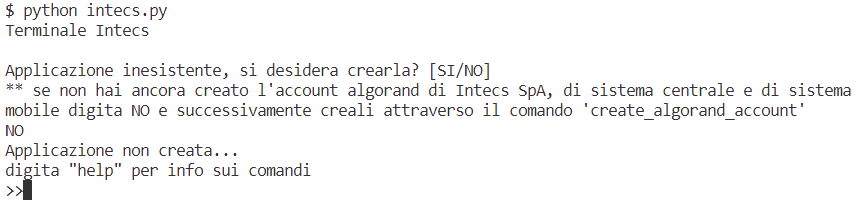
\includegraphics[scale=0.8]{images/Intecs/primo_avvio.png}
% \caption{Primo avvio dell'applicazione}
% \label{fig: intecs_primoavvio_ }
% \end{figure}
Il messaggio "Applicazione inesistente, si desidera crearla? [SI/NO]" viene mostrato ad ogni avvio finché lo smart contract  non verrà creato.
 
\subsection{Generare un account Algorand}\label{generareaccountalgorand}
La creazione di un account Algorand sulla rete TestNet è una procedura molto semplice utilizzando il programma Intecs, ci basta digitare il comando \textit{create\_algorand\_account} [vedi figura \ref{fig: intecs_create_algorand_account}].
\begin{figure}[!h]
\flushleft
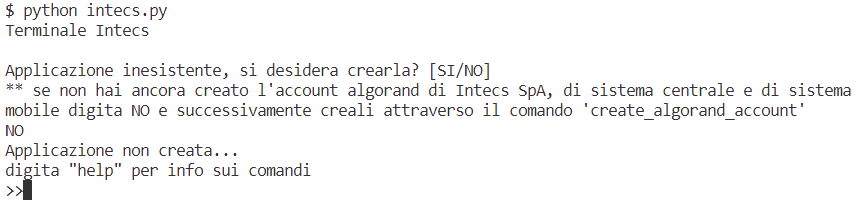
\includegraphics[scale=0.8]{images/Intecs/primo_avvio.png}
\caption{Primo avvio dell'applicazione}
\label{fig: intecs_primoavvio_ }
\end{figure}
\begin{figure}[!h]
\centering
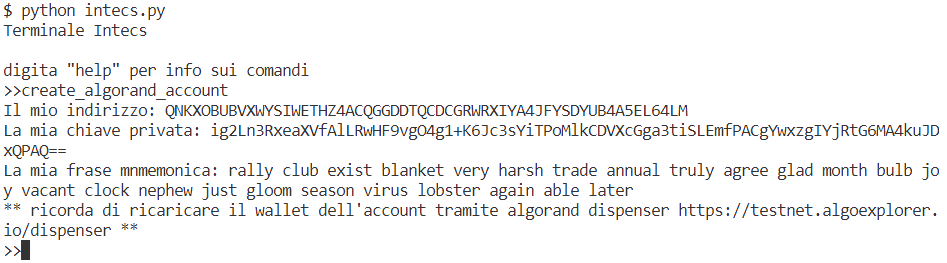
\includegraphics[scale=0.8]{images/Intecs/create_algorand_account.png}
\caption{Creazione di un Algorand account tramite l'interfaccia a linea di comando Intecs}
\label{fig: intecs_create_algorand_account}
\end{figure}\\
Una volta creato l'account, è necessario memorizzare manualmente i tre campi restituiti. Come viene suggerito anche nella fase di creazione dell'account dal programma Intecs, devono essere aggiunti Algos nel Wallet dell'account attraverso l'Algorand Dispenser \cite{algoranddispenser}.

\subsection{Creazione dello smart contract}\label{creazione_smart_contract}
Lo smart contract è un contratto che è possibile creare solamente dopo la creazione dell'account Algorand di Intecs SpA. Successivamente è necessario modificare i valori delle tre variabili globali (intecs\_address, intecs\_privatekey e intecs\_passphrase) del programma intecs.py che si trovano sotto la dichiarazione delle librerie, nelle prime righe del codice. Dopo questa procedura, bisogna creare anche l'account associato al sistema centrale. La figura \ref{fig: intecs_create_smart_contract_} mostra il programma Intecs nella fase di creazione dello smart contract, al termine del quale restituirà l'application-id, un identificatore univoco. Con la creazione dello smart contract è necessario come suggerito anche dall'interfaccia a linea di comando Intecs, settare manualmente l'app-id di sistema centrale, di sistema mobile nei due file config.json, che si trovano rispettivamente nella cartella \textit{sistema\_centrale} e \textit{sistema\_mobile}. La fase di opt-in dell'account Intecs è cruciale perché imposta il valore della variabile globale address\_sistema\_centrale dello smart contract appena creato. La condizione necessaria affinché la creazione di una nuova app vada a buon fine è che l'app corrente sia stata eliminata o che si tratti del primo avvio del programma. In questo modo si evita di avere duplicati di smart contract associati all'account Algorand di Intecs.
\begin{figure}[!h]
\centering
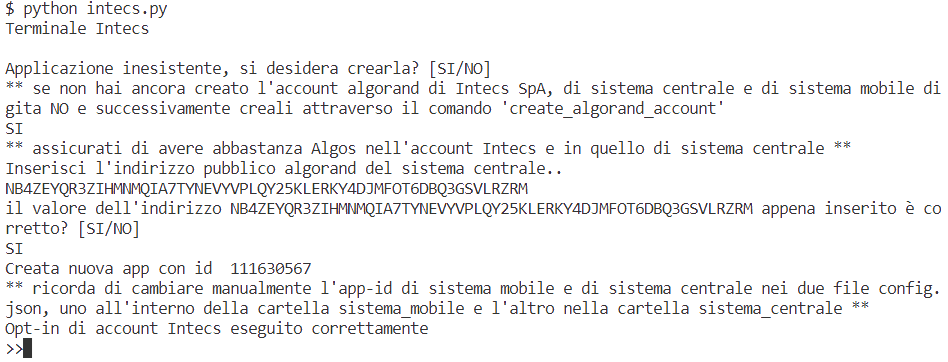
\includegraphics[scale=0.8]{images/Intecs/creazione_smartcontract.png}
\caption{Creazione dello smart contract}
\label{fig: intecs_create_smart_contract_}
\end{figure}

\subsection{Eliminazione dello smart contract}
Il comando \textit{delete\_app} [vedi figura \ref{fig: intecs_delete_smart_contract}] elimina lo smart contract corrente se e solo se il valore di app\_id nel file config.json risulta diverso da 0 e cioè se e solo se esiste. Attraverso il metodo ApplicationDeleteTxn che effettua una transazione alla blockchain si eliminerà lo smart contract. Dopo l'eliminazione sarà di nuovo possibile crearlo con il comando \textit{create\_app} visto nella sezione \ref{creazione_smart_contract}.
\begin{figure}[!h]
\flushleft
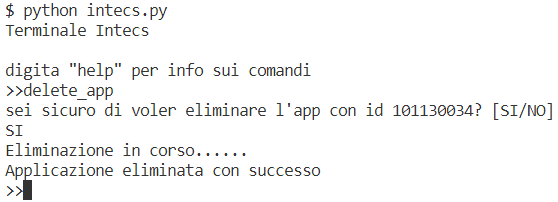
\includegraphics[scale=0.8]{images/Intecs/eliminazione_app.png}
\caption{Eliminazione dello smart contract}
\label{fig: intecs_delete_smart_contract}
\end{figure}

\subsection{Altri comandi}
Vediamo gli altri comandi disponibili con l'interfaccia a linea di comando Intecs.
\begin{itemize}
    \item \textit{app-id}: restituisce l'indice (app-id) univoco associato allo smart contract. Il funzionamento è semplice: si legge il valore della chiave 'app\_id' nel file config.json e si restituisce. Se il valore è impostato a 0 significa che l'applicazione non è mai stata creata oppure è stata eliminata e non è quindi più esistente.
    \item \textit{set\_account\_sistemacentrale}: serve per cambiare il valore della variabile globale address\_sistema\_centrale dello smart contract e di sistema\_centrale\_address nel file config.json. La procedura di modifica può essere eseguita esclusivamente dall'account Algorand di Intecs.
    \item \textit{address\_sistemacentrale}: restituisce, se esiste, il valore dell'indirizzo Algorand del sistema centrale. Semplicemente si effettua una lettura del valore della chiave "sistema\_centrale\_address" nel file config.json per poi restituirla; se il valore è impostato su stringa vuota ("") significa che l'applicazione non è mai stata creata.
    \item \textit{exit}: comando usato per chiudere correttamente il programma.
    \item \textit{clear}: ripulisce la schermata del programma cancellando ogni scritta presente.
    \item \textit{help}: restituisce la lista di tutti i comandi disponibili con una piccola didascalia per rendere più chiaro il funzionamento di ognuno di questi.
\end{itemize}

\subsection{Tabella riassuntiva dei comandi}
\resizebox{\textwidth}{!}{%
\begin{tabular}{llllll}
\toprule
{\bfseries Comando} & {\bfseries Sintassi} & {\bfseries
Esempio}\\
\midrule
create\_app & create\_app & create\_app \\
\midrule
app-id & app-id & app-id \\
\midrule
delete\_app & delete\_app & delete\_app \\
\midrule
set\_account\_sistemacentrale & set\_account\_sistemacentrale <address> & set\_account\_sistemacentrale 597c28c381ef1fee \\
\midrule
create\_algorand\_account & create\_algorand\_account & create\_algorand\_account \\
\midrule
address\_sistemacentrale & address\_sistemacentrale & address\_sistemacentrale \\
\midrule
exit & exit & exit \\
\midrule
clear & clear & clear \\
\bottomrule
\end{tabular}}


\chapter{Simulazione del sistema di rilevazione}\label{6.simulazione del progetto}
\section{Creazione dello smart contract}\label{creazionesmartcontract}
Prima di poter creare lo smart contract è necessario generare l'account Algorand Intecs SpA con il quale, potremo creare lo smart contract e richiamare i metodi di quest'ultimo. Per la creazione di un account è sufficiente avviare il programma intecs.py presente nella cartella \textit{intecs}. Al primo avvio, digitiamo NO in quanto bisogna prima creare gli account Algorand che ci serviranno. Verrà quindi mostrata la schermata in figura \ref{fig: intecs_primoavvio }.
\begin{figure}[!h]
\flushleft
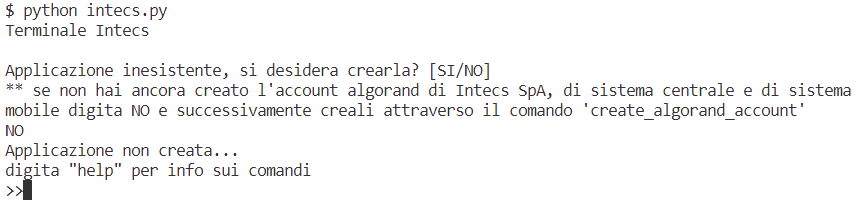
\includegraphics[scale=0.8]{images/Intecs/primo_avvio.png}
\caption{Primo avvio dell'interfaccia a linea di comando Intecs}
\label{fig: intecs_primoavvio }
\end{figure}\\
Attraverso il comando \textit{create\_algorand\_account} possiamo creare gli account Algorand.
\begin{figure}[!h]
\centering
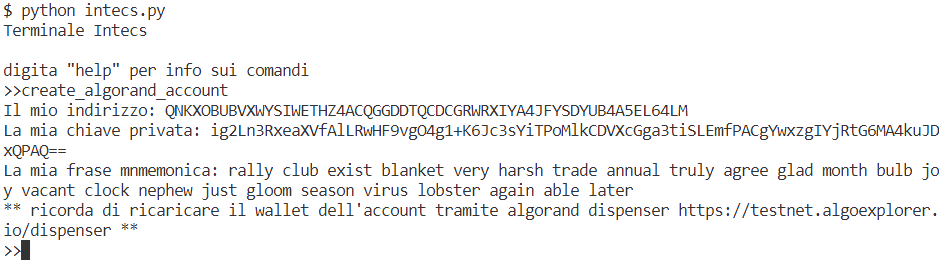
\includegraphics[scale=0.8]{images/Intecs/create_algorand_account_2.png}
\caption{Creazione degli account Algorand}
\label{fig: cli_creazioneaccount2 }
\end{figure}\\
Notiamo immediatamente dalla figura \ref{fig: cli_creazioneaccount2 } che la creazione di un account Algorand genera tre campi: l'indirizzo pubblico, la chiave privata e la mnemonica. E' necessario memorizzare manualmente questi dati visto che serviranno nelle fasi successive. Ricordiamo anche, che dopo la creazione di un account Algorand, il Wallet dovrà essere caricato con Algos (la moneta della TestNet) sfruttando l'Algorand Dispenser. Il comando \textit{create\_algorand\_account} va richiamato per creare l'account Intecs SpA, del sistema centrale e per ogni sistema mobile esistente. Nel nostro esempio consideriamo un solo sistema mobile. Una volta creato anche l'account di Intecs SpA chiudiamo il programma sfruttando il comando \textit{exit} per avere modo di modificare i valori delle variabili globali dell'account Algorand di Intecs (intecs\_address, intecs\_privatekey e intecs\_passphrase) che si trovano nelle prime righe del codice del programma subito dopo le librerie. Riavviamo nuovamente l'interfaccia a linea di comando intecs.py per effettuare finalmente l'operazione di creazione dello smart contract come nell'immagine \ref{fig: intecs_create_smart_contract}. 
\begin{figure}[!h]
\centering
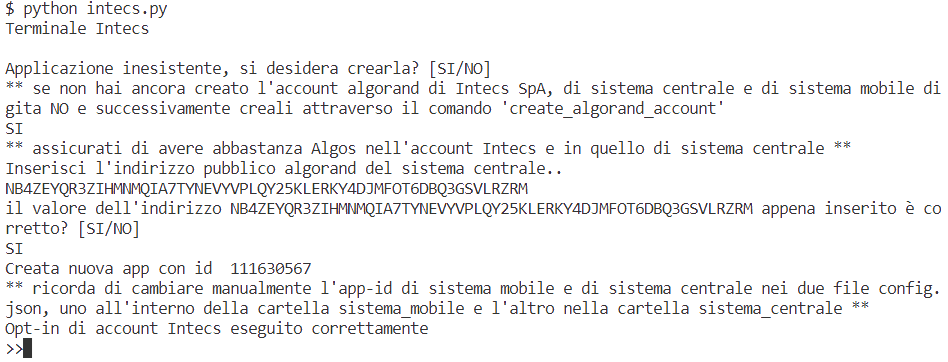
\includegraphics[scale=0.8]{images/Intecs/creazione_smartcontract.png}
\caption{Creazione dello smart contract}
\label{fig: intecs_create_smart_contract}
\end{figure}\\
L'operazione ha generato uno smart contract con il seguente ID: 111630567. Collegandosi al portale AlgoExplorer \cite{algoexplorer_testnet} e inserendo l'identificatore (ID) dello smart contract, possiamo verificare la corretta creazione di quest'ultimo.

\section{Setting dei file JSON}
Dopo la creazione dello smart contract è necessario andare a settare i valori degli account Algorand nel codice del programma di sistema centrale, di sistema mobile e di Cli v2. Più nel dettaglio:
\begin{itemize}
    \item apriamo il file info\_algorand.json presente nella cartella \textit{sistema\_centrale} per settare i tre parametri dell'indirizzo Algorand di sistema centrale (sistema\_centrale\_address, sistema\_centrale\_privatekey e sistema\_centrale\_passphrase) e il valore di app\_id, che sono stati generati nella sezione \ref{creazionesmartcontract}. Se non ricordiamo l'app-id associato allo smart contract creato, possiamo recuperarlo con il programma intecs.py richiamando il comando \textit{app-id}.
    \item apriamo il file info\_algorand.json presente nella cartella \textit{sistema\_mobile} per settare i tre parametri dell'indirizzo Algorand di sistema mobile (sistema\_mobile\_address, sistema\_mobile\_privatekey e sistema\_mobile\_passphrase) e il valore di app\_id  generati nella sezione \ref{creazionesmartcontract}. Nel caso in cui non ci si ricordi l'identificatore (id) associato allo smart contract creato, possiamo avviare il programma intecs.py e richiamare il comando \textit{app-id}, il quale restituirà il valore associato all'applicazione (smart contract).
    \item nella cartella \textit{cli v2} apriamo il file config.json e settiamo il valore della chiave sistema\_centrale\_address con l'indirizzo Algorand pubblico generato nella sezione \ref{creazionesmartcontract}.
\end{itemize}
Tutti i settaggi sono stati ora impostati correttamente.

\section{Avvio del programma}
L'avvio del programma è un'operazione che può essere istanziata automaticamente attraverso il docker-compose.yml con il comando \textit{docker-compose up --build}. Per sfruttare questa opzione è necessario aver installato sia Docker che Docker Compose. Nel qual caso si vogliano avviare manualmente le singole componenti senza far uso di Docker, è necessario prima di tutto modificare il campo \textit{host} delle configurazioni TCP, inserendo indirizzi IP validi al posto dei nomi di dominio impostati. Spieghiamo meglio questo concetto prendendo come esempio la configurazione utilizzata per la comunicazione TCP con il sistema mobile, ci riferiamo cioè al programma sistemacentrale.py, che gestisce la ricezione dei file zip e JSON. Notiamo che l'host, non è stato dichiarato sfruttando un indirizzo IP ma direttamente con il nome del servizio "sistemacentrale" dichiarato nel file docker-compose.yml il quale si riferisce al programma sistemacentrale.py e cioè al container del sistema centrale. Quest'operazione è consentita grazie a Docker Compose. Infatti quando nel docker-compose.yml aggiungiamo un servizio, non facciamo altro che definire un nuovo container e il nome stesso del container rappresenterà il suo nome di dominio.
\begin{pythoncode}
#configurazione Server TCP con Sistema Mobile (ricezione zip e json)
host_sm = "sistemacentrale"
port_sm = 12370
\end{pythoncode}
Questa proprietà vale però solo all'interno della rete Docker avviando il programma con docker-compose.yml. Nel qual caso si vogliano avviare le singole componenti manualmente (senza usare Docker) dobbiamo modificare tutte le varie configurazioni ed utilizzare indirizzi IP al posto dei nomi dei container per il campo \textit{host}. Le componenti poi dovranno essere avviate nel seguente ordine: sistemacentrale.py, sistemamobile.py e stazioneriferimento.py. In figura \ref{fig: sistemacentraleoutput } mostriamo l'output del sistema centrale subito dopo il suo avvio.
\begin{figure}[!h]
\flushleft
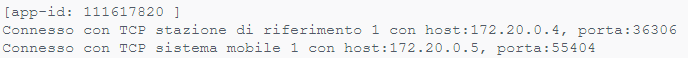
\includegraphics[scale=1.1]{images/simulazione/outputsistemacentrale.png}
\caption{Output dopo l'avvio del sistema centrale}
\label{fig: sistemacentraleoutput }
\end{figure}\\
Dopo aver avviato le tre componenti appena citate deve essere avviato il programma antenna che genererà il timestamp e lo invierà al sistema mobile e alla stazione di riferimento [vedi figura \ref{fig: antennaoutput }].
\begin{figure}[!h]
\flushleft
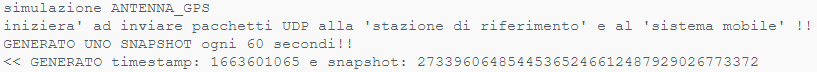
\includegraphics[scale=1.0]{images/simulazione/antennaoutput}
\caption{Output di antenna dopo l'invio di uno snapshot}
\label{fig: antennaoutput }
\end{figure}\\
L'output del terminale del sistema mobile conterrà la notifica di ricezione dello snapshot e del timestamp e mostrerà lo snapshot e i dati di posizioni appena generati [vedi figura \ref{fig: sistemamobile }].
\begin{figure}[!h]
\flushleft
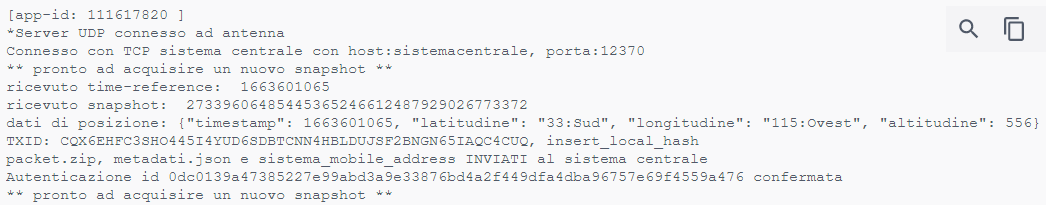
\includegraphics[scale=0.8]{images/simulazione/outputsistemamobile.png}
\caption{Schermata del sistema mobile}
\label{fig: sistemamobile }
\end{figure}\\
Anche il terminale della stazione di riferimento, avrà un output molto simile a quello del sistema mobile, conterrà infatti la notifica di ricezione del timestamp e dello snapshot e mostrerà lo snapshot e i dati di posizione appena generati [vedi figura \ref{fig: sistema_centrale6 }].\\
\begin{figure}[!h]
\flushleft
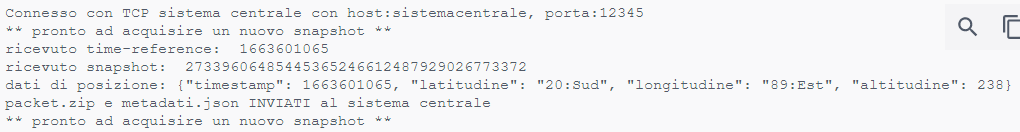
\includegraphics[scale=0.8]{images/simulazione/outputstazioneriferimento.png}
\caption{Schermata della stazione di riferimento}
\label{fig: sistema_centrale6 }
\end{figure}\\
Come ultima operazione, il sistema mobile e la stazione di riferimento inviano entrambi il file zip e il file JSON al sistema centrale sfruttando la comunicazione TCP. Dopo la ricezione di questi documenti, il sistema mobile invia anche il proprio indirizzo pubblico Algorand [vedi figura \ref{fig: sistema_centrale7 }]. 
\begin{figure}[!h]
\flushleft
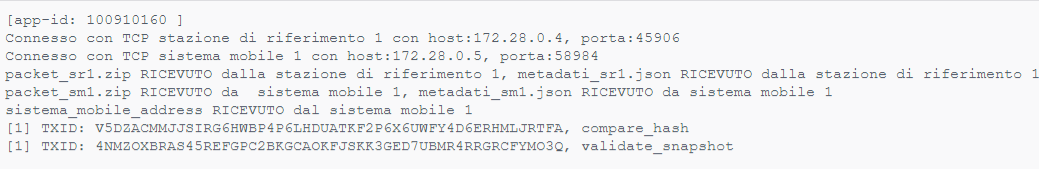
\includegraphics[scale=0.8]{images/simulazione/sistema_centrale.png}
\caption{Schermata del sistema centrale}
\label{fig: sistema_centrale7 }
\end{figure}
A questo punto, apriamo il programma Cli e sfruttiamo il comando \textit{stampa\_lista\_id} per vedere che l'id associato allo snapshot ricevuto poco fa dal sistema mobile ed inviato al sistema centrale è disponibile alla visualizzazione. Possiamo anche visualizzare alcune informazioni utili come la data e l'ora di ricezione dello snapshot da parte del sistema mobile e se lo snapshot è stato certificato correttamente. Quest'ultimo campo è rappresentato con un valore booleano True/False, ricordando che il valore booleano della validazione è settato a False se lo snapshot catturato dal sistema mobile e dalla stazione di riferimento non risultano equivalenti [vedi figura \ref{fig: sistema_centrale8 }].
\begin{figure}[!h]
\flushleft
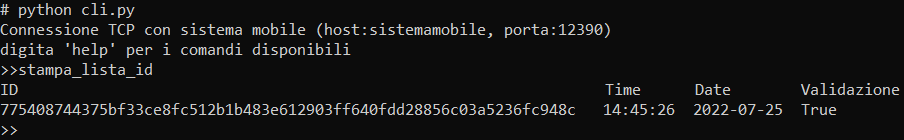
\includegraphics[scale=0.8]{images/simulazione/cli1.png}
\caption{Un primo esempio dell'interfaccia a linea di comando Cli}
\label{fig: sistema_centrale8 }
\end{figure}\\
Sfruttando il comando \textit{info\_id} e utilizzando come parametro l'id restituito da \textit{stampa\_lista\_id} possiamo avere accesso a tutte le informazioni associate allo snapshot corrispondente all'id passato. Diventa utile per ricercare un particolare snapshot catturato dal sistema mobile e controllare dove si trovava il sistema mobile ad una certa ora di un dato giorno [vedi figura \ref{fig: sistema_centrale9 }].
\begin{figure}[!h]
\flushleft
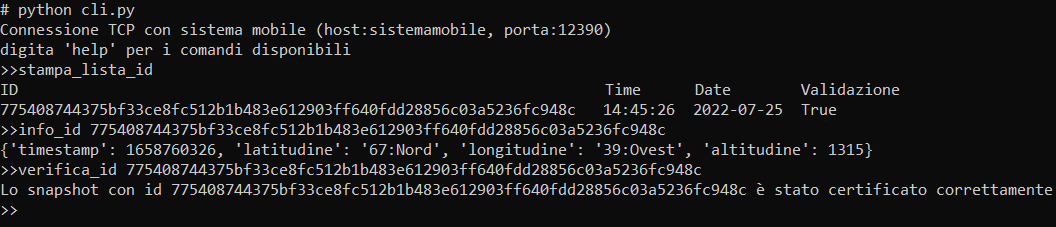
\includegraphics[scale=0.7]{images/simulazione/cli2.png}
\caption{Un secondo esempio dell'interfaccia a linea di comando Cli}
\label{fig: sistema_centrale9 }
\end{figure}

\chapter{Conclusioni}\label{7.conclusioni}
E' interessante mostrare un'implementazione alternativa che è stata analizzata solo concettualmente, per rimanere nella filosofia di decentralizzazione che è intrinseca nella blockchain. La soluzione propone di sfruttare una tecnologia decentralizzata anche per la memorizzazione dei dati. Nel progetto implementato, il sistema centrale archivia i file zip e JSON ricevuti dal sistema mobile e dalla stazione di riferimento internamente. Per evitare il fenomeno del collo di bottiglia, una soluzione sarebbe potuta essere quella di memorizzarli su IPFS, un file system decentralizzato, introducendo quindi una ridondanza sui file.

\section{IPFS (Interplanetary File Sistem)}
L'IPFS \cite{ipfs_homepage}, acronimo di InterPlanetary File System, è un file system decentralizzato, implementato con una rete peer-to-peer. Si tratta di un sistema per l'archiviazione e la condivisione di dati. Quando si aggiunge un file a IPFS, il file viene suddiviso in blocchi più piccoli, sottoposto ad una funzione crittografica di hash e il risultato ottenuto è un'impronta digitale unica chiamata CID (content identifier). Il CID è un identificatore permanente del file. Quando i nodi cercano quel file, chiedono ad altri nodi chi sta archiviando il contenuto a cui fa riferimento il CID del file. Quando visualizzano o scaricano il file, ne memorizzano una copia nella cache e diventano un altro fornitore del contenuto, fino a quando la cache non viene svuotata. Un nodo può bloccare il contenuto per conservarlo (e fornirlo) per sempre, o scartare il contenuto che non utilizza da un po' di tempo per risparmiare spazio. Questo significa che ogni nodo della rete archivia solo il contenuto a cui è interessato, oltre ad alcune informazioni di indicizzazione che aiutano a capire quale nodo sta archiviando cosa. Aggiungendo una nuova versione di quel file a IPFS, il suo hash crittografico sarà diverso e quindi si otterrà un nuovo CID. Ciò significa che i file archiviati su IPFS sono resistenti alla manomissione e alla censura: qualsiasi modifica ad un file non sovrascrive l'originale e i blocchi comuni tra i file possono essere riutilizzati per ridurre al minimo i costi di archiviazione \cite{ipfs}.

\subsection{Implementazione}
Nel progetto implementato, quando il sistema centrale riceve i file zip e JSON riferiti a uno snapshot, calcola l'id (cioè l'hash del file zip), crea il record <id, path del file zip> da salvare nell'object\_storage.json e il record <id, path del file json> da memorizzare all'interno di metadati.json. Introducendo la tecnologia di IPFS, non appena il sistema centrale riceve i file zip e JSON, li aggiunge al file system di IPFS. Il caricamento restituirà un CID (content identifier) per ognuno di questi file caricati. Basterà leggermente modificare il record da salvare nell'object\_storage.json con l'aggiunta di un campo che conterrà il valore del CID in questo modo: <id, path del file zip, CID>. La stessa modifica sarà necessaria anche per il record  caricato nel file metadati.json.

\section{Tecnologia e Ambiente}
\subsection{Sostenibilità di Algorand}
La tecnologia, intesa come progresso tecnologico, ha fatto registrare un forte impatto sulla natura. Al contrario di cento o duecento anni fa, però, oggi ne abbiamo la piena consapevolezza: adottare approcci sostenibili per raggiungere un obiettivo green è diventato un dovere che coinvolge tutti. Buona parte dell’energia viene perduta a causa dell’impiego di tecnologie poco efficienti, per sprechi ed usi impropri. Le prestazioni tecnologiche delle blockchain dipendono dai loro protocolli di consenso. All'inizio di questo percorso tecnologico, i cosiddetti protocolli di consenso Proof of Work (PoW) hanno alimentato la prima generazione di blockchain, con il merito di mostrare l'esistenza del valore nativo digitale ma allo stesso tempo hanno condotto una battaglia computazionale planetaria per convalidare il prossimo blocco di dati, con uno spreco di energia inaccettabile. Infatti, come suggerisce la parola stessa "Proof of Work", mostrare un impegno personale nell'ecosistema attraverso l'allocazione di risorse computazionali ed energetiche è al centro di questo meccanismo di consenso. Tuttavia, le blockchain che funzionano su PoW non riescono a soddisfare la promessa di scalabilità, decentralizzazione, velocità delle transazioni e costi, finiscono per fare affidamento su fattorie computazionali centralizzate energeticamente inefficienti. È qui che Algorand interviene grazie al brillante lavoro del Professor Silvio Micali, una nuova orchestrazione di calcolo distribuito, crittografia e teoria dei giochi all'avanguardia ha trasformato le aspirazioni delle blockchain originali nel nuovissimo protocollo di consenso Algorand Pure Proof of Stake (PPoS). La Pure Proof of Stake è energeticamente sostenibile? Per inquadrare correttamente questa domanda è stata proposta una stima approssimativa del consumo energetico di PPoS e di un'impronta di carbonio. Poiché la stima dell'impronta di carbonio dipende strettamente dagli scenari di generazione di energia e dal grado locale di fonti rinnovabili, è necessario affrontare prima un'altra metrica critica: la Finalized Transaction Energy per Validator, ovvero la quantità media di energia spesa da un validatore per finalizzare una singola transazione e aggiungerla al libro mastro distribuito comune (Distributed Ledger). Nell'esempio consideriamo come risorsa hardware del validatore un Raspberry Pi 4, che ha una potenza per ogni nodo di: 
\begin{displaymath}
P = 7,2 [W]
\end{displaymath}
e un numero di transazioni finalizzate al secondo (considerando l'algoritmo di Pure Proof of Stake) pari a:
\begin{displaymath}
TPS = 1000 [txn/s].
\end{displaymath}

Evitiamo di mostrare i calcoli e concludiamo dicendo che in media, l'energia spesa per convalidare una transazione sarà:

\begin{displaymath}
E = \frac{P}{TPS} = 2 \: \frac{\mu Wh}{txn}
\end{displaymath}

\subsubsection{Sostenibilità e scalabilità}
Come passaggio finale, mostriamo il grafico \ref{fig: graficoconsumi } che rappresenta l'intera quantità di energia spesa dai diversi protocolli per raggiungere il consenso sul blocco successivo e mantenere la blockchain sicura, valutando l'energia complessiva spesa dall'intera rete per la conferma di una singola transazione.
\begin{figure}[!h]
\centering
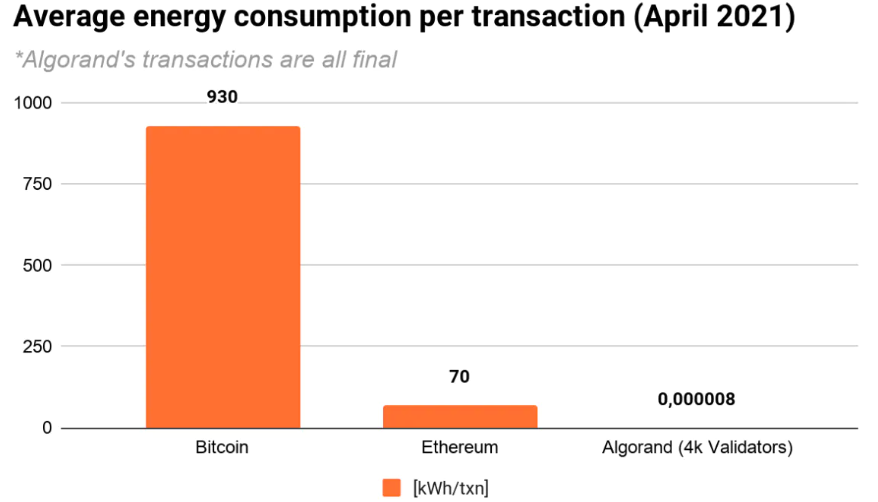
\includegraphics[scale=0.6]{images/schema_consumo.png}
\caption{Grafico dei consumi \cite{algorand_ambiente}}
\label{fig: graficoconsumi }
\end{figure}\\
Quindi, supponendo blocchi interi, mostriamo l'energia consumata dalle varie blockchain:
\begin{description}
    \item [Bitcoin] \begin{displaymath} E = 930 \: \frac{kWh}{txn} \end{displaymath}
    \item [Ethereum] \begin{displaymath} E = 70 \: \frac{kWh}{txn} \end{displaymath}
    \item [Algorand] \begin{displaymath} E = 0,000008 \: \frac{kWh}{txn} \end{displaymath}
\end{description}
Anche in questo caso, abbiamo evitato di appesantire il lettore con i calcoli. Per eventuali approfondimenti si rimanda all'articolo originale \cite{algorand_ambiente}.

\section{Sviluppi Futuri}

\subsection{Uso dei token}
Sicuramente un aspetto da non sottovalutare è quello relativo alla sicurezza dei sistemi mobili quando comunicano con lo smart contract. Nel progetto sviluppato nessuno può spacciarsi per un sistema centrale, infatti l'indirizzo pubblico di quest'ultimo viene memorizzato nella variabile globale \textit{Address Sistema Centrale} all'interno dello smart contract nella fase di opt-in di Intecs. Quando i metodi dello smart contract, costruiti appositamente per il sistema centrale, vengono chiamati (ci riferiamo a compare\_hash e validate\_snapshot), controllano che l'indirizzo mittente sia proprio uguale a \textit{Address Sistema Centrale}. Il problema risiede nel fatto che chiunque potrebbe fare opt-in allo smart contract e spacciarsi per un sistema mobile per richiamare il metodo \textit{insert\_local\_hash}. L'uso di token (gettoni) rappresenterebbe una soluzione al problema, in particolare l'uso di token che prendono il nome di \textit{asset token frozen} (token che si possono revocare), distribuiti dall'account Intecs ai vari account Algorand dei sistemi mobile come se fossero una sorta di "chiave" di accesso. Quando il sistema mobile invoca il metodo \textit{insert\_local\_hash} dello smart contract, mostrando il suo token, certifica che lui ha il permesso di fare quell'operazione. Detto in altri termini, dobbiamo far si che sia Intecs a poter dare l'ok ai sistemi mobile e questa implementazione la posso fare costruendo un account Intecs che crea token e ne dona uno ad ogni sistema mobile da usare come certificazione.

\section{Conclusioni}
Ritengo sia stato molto stimolante lavorare a questo progetto, visto che si tratta di una tecnologia in continua evoluzione che risulterà sempre più utilizzata nel futuro. Il progetto in sé, rappresenta un prototipo, per far capire quali possano essere le potenzialità della tecnologia blockchain e degli smart contract. Alcuni parti del progetto sono sicuramente migliorabili, ad esempio risulta macchinoso dover modificare manualmente i file di configurazione (JSON) ogni qualvolta si abbia la necessità di creare una nuova applicazione o di cambiare l'indirizzo Algorand pubblico del sistema centrale. Questa parte richiederebbe un'ulteriore approfondimento, che si potrebbe risolvere con l'utilizzo di un secondo smart contract gestito da Intecs SpA attraverso l'interfaccia a linea di comando intecs.py che memorizza l'indirizzo Algorand del sistema centrale e dell'application-id. Con tale sistema, ogni volta che viene modificato uno di questi valori, il programma intecs.py invia un segnale ai vari dispositivi per richiedere una nuova lettura delle variabili da questo smart contract e l'aggiornamento dei file di configurazione di tipo JSON.

\chapter*{Ringraziamenti}
\addcontentsline{toc}{chapter}{Ringraziamenti}
\chaptermark{Ringraziamenti}
\rhead{}
Desidero ringraziare il mio tutore aziendale Simone Gianfranceschi che mi ha dato l'opportunità di svolgere questo tirocinio così interessante insieme a Giovanni Iovino, il quale mi ha seguito durante tutto il percorso. Un grazie anche al mio tutore accademico, la professoressa Laura Ricci per la disponibilità e la gentilezza dimostratomi. Ringrazio anche la mia famiglia, la mia ragazza Silvia e i miei amici che mi hanno sostenuto in questo cammino tortuoso, non sempre facile. 
\\
\\
\\
\textit{"C’è una forza motrice più forte del vapore, dell’elettricità e dell’energia atomica: la volontà."}
\begin{flushright}
\textit{Albert Einstein}
\end{flushright}

\printbibliography[
heading=bibintoc,
title={Bibliografia}
]

% \begin{refsection}[references2.bib]
% \nocite{*}
% \printbibliography[
% heading=bibintoc,
% keyword={capitolo6Lorenzo},
% title={Bibliografia appendice C}
% ]
% \end{refsection}


\end{document}
